% =====================================================================
%  Supplementary material — Illex illecebrosus population genomics
%  Diagnostic figures + detail tables. Build: make supp  (or pdflatex+bibtex)
% =====================================================================
\documentclass[11pt]{article}
\usepackage[utf8]{inputenc}
\usepackage[T1]{fontenc}
\usepackage{lmodern}
\usepackage[margin=1in]{geometry}
\usepackage{graphicx}
\usepackage{booktabs}
\usepackage{amsmath}
\usepackage{amssymb}
\usepackage{longtable}
\usepackage[round]{natbib}
\usepackage{xcolor}
\usepackage[colorlinks=true,allcolors=blue]{hyperref}
\usepackage{cleveref}

\graphicspath{{supp_figures/}}
\newcommand{\illex}{\textit{Illex illecebrosus}}
\newcommand{\coin}{\textit{I.\ coindetii}}
\newcommand{\Fst}{F_\mathrm{ST}}
\newcommand{\dxy}{d_\mathrm{xy}}

% number supplementary floats S1, S2, ...
\renewcommand{\thefigure}{S\arabic{figure}}
\renewcommand{\thetable}{S\arabic{table}}

\title{\textbf{Supplementary material}\\[2pt]
  Population genomics of the northern shortfin squid \textit{Illex illecebrosus}}
\author{}
\date{\today}

\begin{document}
\maketitle

\section*{Supplementary figures}

\begin{figure}[h]\centering
  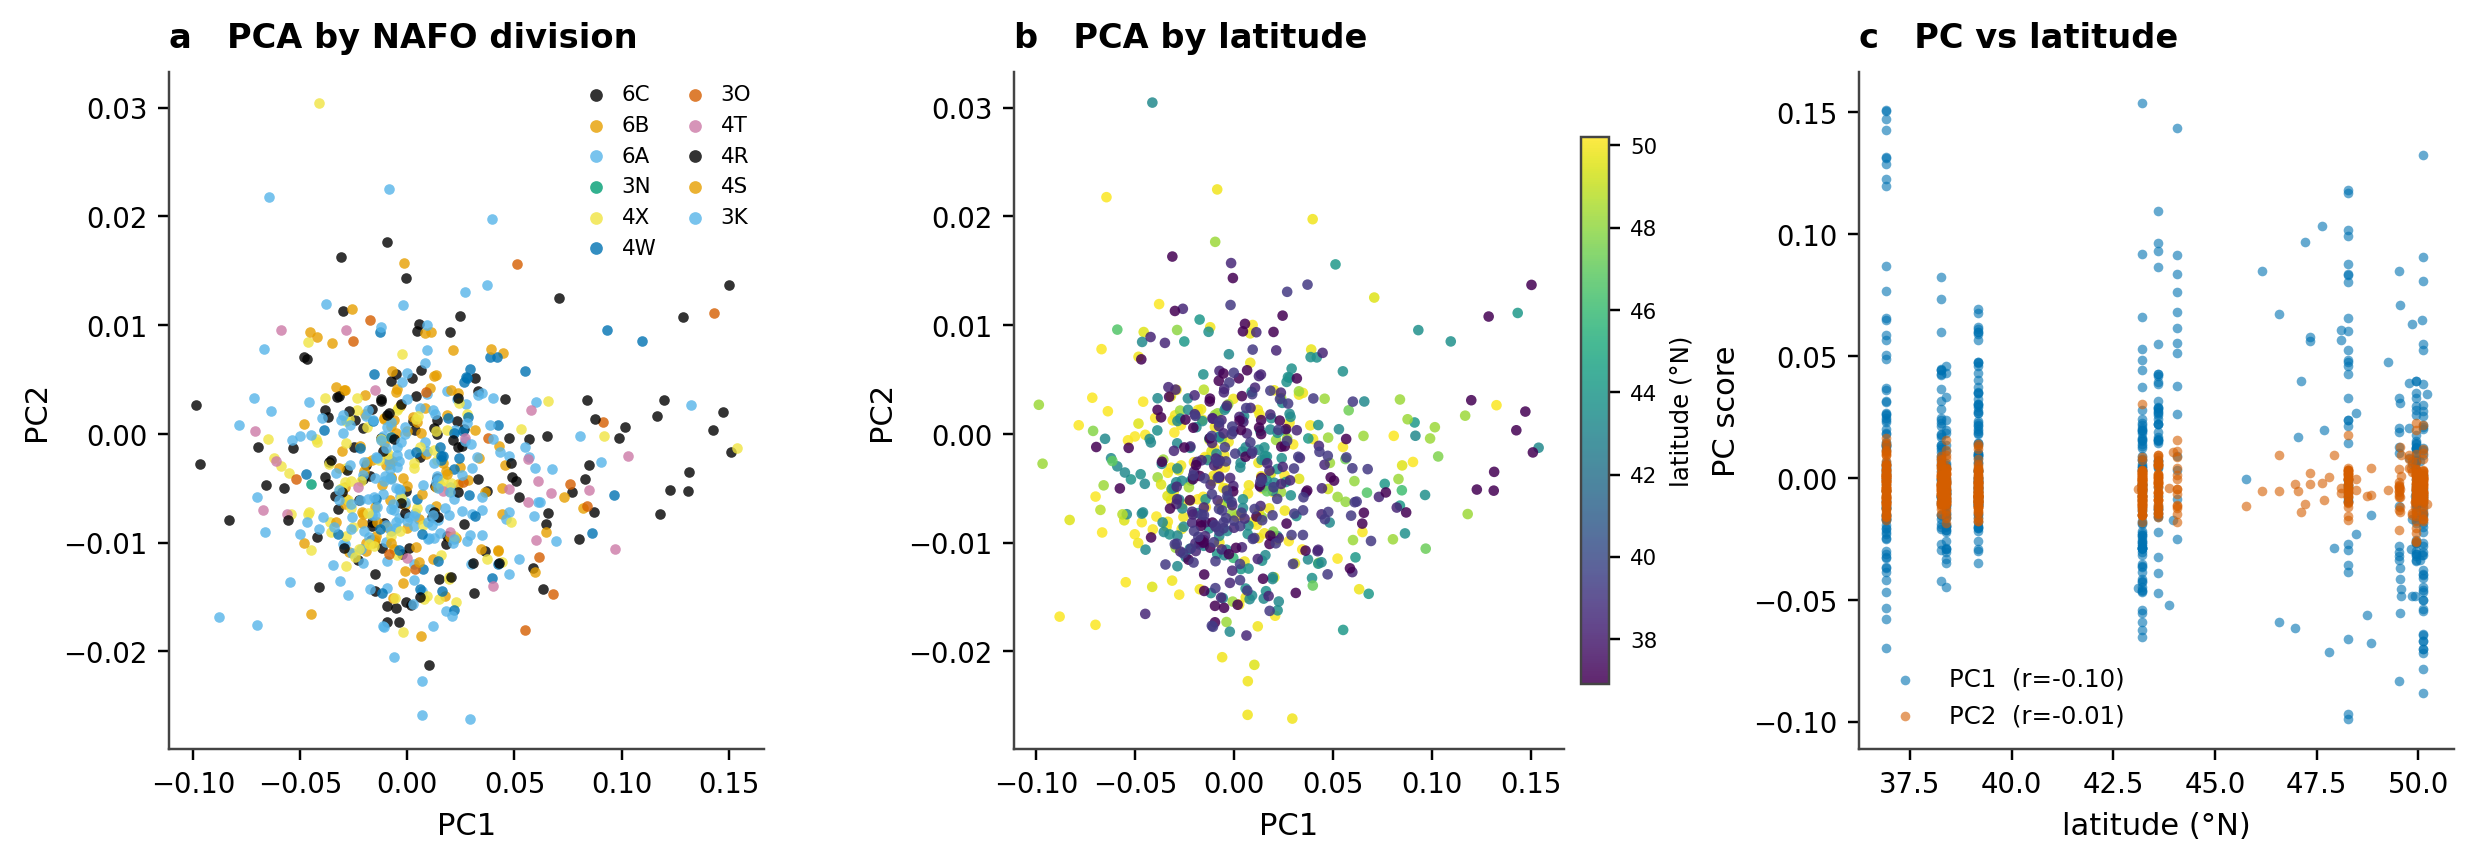
\includegraphics[width=\linewidth]{figS1_pca_geography.png}
  \caption{\textbf{The autosomal-PCA spread is not geographic structure.} Genome-wide PCA
    (autosomes; chromosome~2, chromosome~42 and the Z excluded), $n=621$ individuals.
    (a)~Coloured by NAFO sampling division and (b)~by latitude, the divisions and the
    latitudinal gradient are fully intermixed across PC space, with no clustering by origin.
    (c)~PC scores plotted against latitude show no relationship (Pearson $r=-0.10$ for PC1,
    $r=-0.01$ for PC2). The dispersion along the minor PC axis in main-text Fig.~2 is carried by a handful
    of individuals ($\sim$9 samples account for $>$80\% of the PC2 variance) and tracks neither division nor
    latitude nor sequencing coverage; a KING-robust screen finds no cryptic relatedness among them, so it is
    a minor-axis artifact rather than population subdivision, consistent with genome-wide $\Fst\approx0$.}
  \label{sfig:pcageo}
\end{figure}

\begin{figure}[h]\centering
  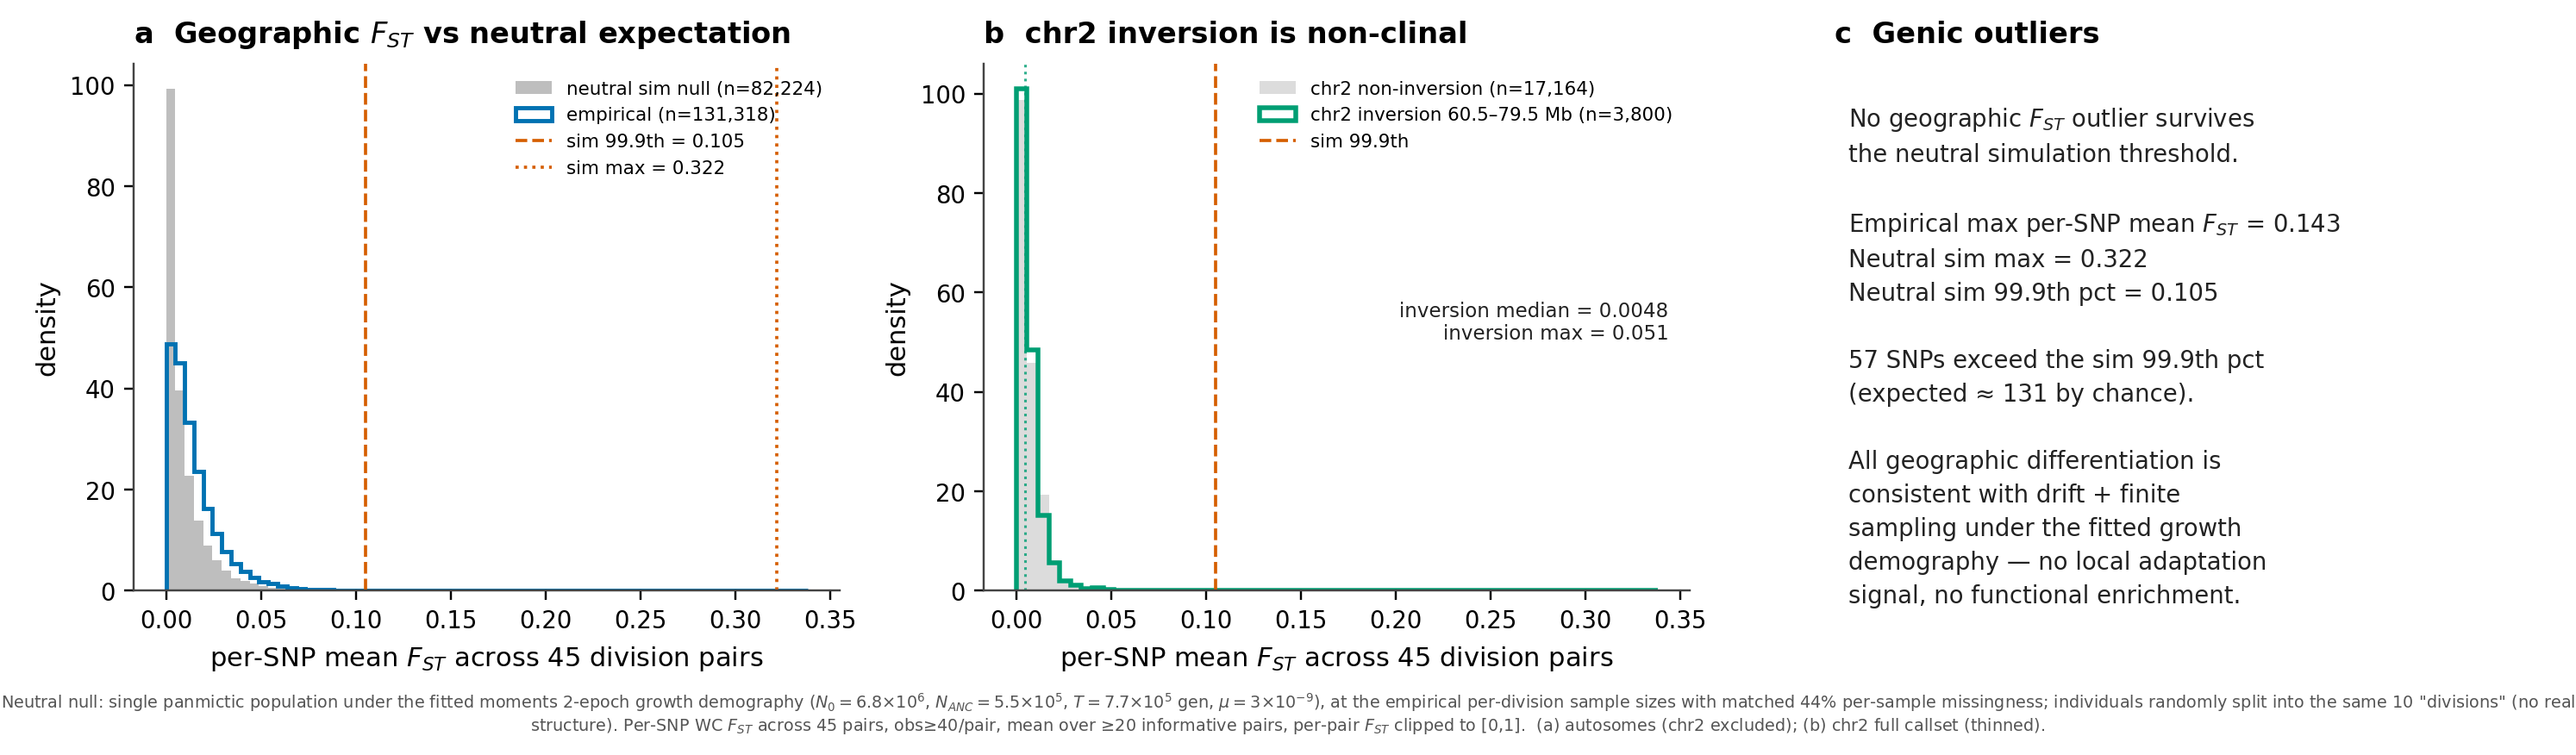
\includegraphics[width=\linewidth]{figS2_fst_expanded.png}
  \caption{\textbf{No geographic differentiation beyond genetic drift; no local adaptation signal.} Per-SNP
    Weir--Cockerham $\Fst$ across all 45 NAFO-division pairs (well-genotyped sites, $\geq$40 observed
    haplotypes per pair; per-SNP mean over $\geq$20 informative pairs). \textbf{(a)}~The empirical distribution
    (blue) lies entirely within a coalescent neutral null (grey), which is a single panmictic population
    simulated under the fitted growth demography ($N_0=6.8\times10^{6}$, $N_\mathrm{ANC}=5.5\times10^{5}$,
    $\mu=3\times10^{-9}$) at the empirical per-division sample sizes with the matched 44\% missingness, split
    at random into ten ``divisions''. Empirical max $\Fst=0.143$ vs neutral max $0.322$; only 57 SNPs exceed
    the neutral 99.9th percentile ($0.105$) against $\approx$131 expected by chance, fewer than the false-positive rate. Drift, finite sampling and missingness fully explain the observed differentiation.
    \textbf{(b)}~On chromosome~2, the inverted region (green) is geographically indistinguishable from the
    collinear remainder (median $\Fst\approx0.005$), so the inversion is non-clinal and its $\Fst\approx0.37$ is between karyotypes, not geography. \textbf{(c)}~No SNP survives the neutral threshold, so a scan for
    local adaptation that the diversity-based sweep tests could miss returns no candidates. (The autosomal
    panel samples a fixed 400~kb window per chromosome; the distribution/threshold conclusion is robust, but a
    genome-wide genic-outlier scan would require per-chromosome $\Fst$ on the full callsets.)}
  \label{sfig:fstsnp}
\end{figure}

\begin{figure}[h]\centering
  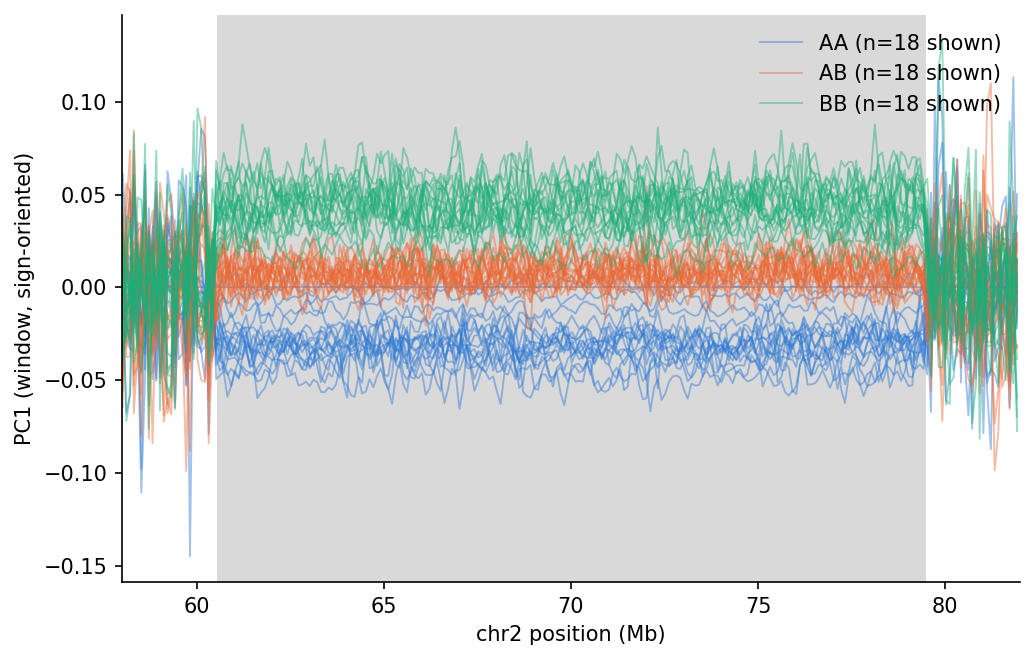
\includegraphics[width=.7\linewidth]{figS3_winpca.png}
  \caption{\textbf{Windowed PCA across chromosome~2} localising the differentiated block.
    [Regeneration note. Window coordinates to be corrected in the final version.]}
  \label{sfig:winpca}
\end{figure}

\begin{figure}[h]\centering
  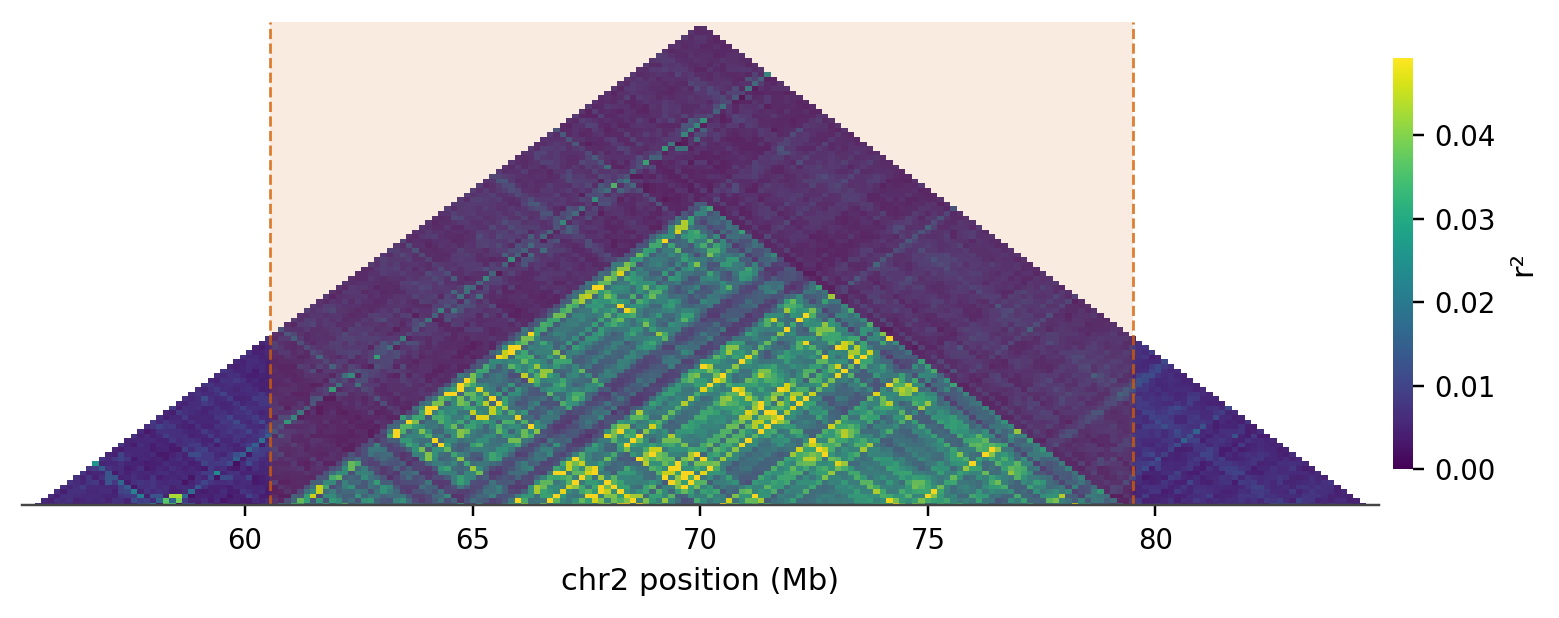
\includegraphics[width=.6\linewidth]{figS4_ld_triangle.png}
  \caption{\textbf{Linkage disequilibrium across the chromosome-2 inversion.} Mean genotype $r^2$ between SNPs, binned along chr2:55--85~Mb, pooling all 633 individuals. Dashed lines and shading mark the breakpoints (60.54 and 79.50~Mb). A block of elevated linkage disequilibrium spans exactly the inverted body and stops at both breakpoints, while the flanking collinear sequence shows only background values. Mean $r^2$ between SNPs more than 1~Mb apart is 3.5 times higher inside the inversion than in its flanks (0.0056 vs 0.0016; Supplementary Fig.~S24). This long-range association arises because the few near-fixed differences between arrangements are all correlated with karyotype, and it is the direct signature of suppressed recombination between arrangements. Recombination within arrangements is not suppressed at the scale of the $\sim$19-kb windows used by the recombination map, which is why the inversion is shown here rather than in Supplementary Fig.~S12.}
  \label{sfig:ld}
\end{figure}

\begin{figure}[h]\centering
  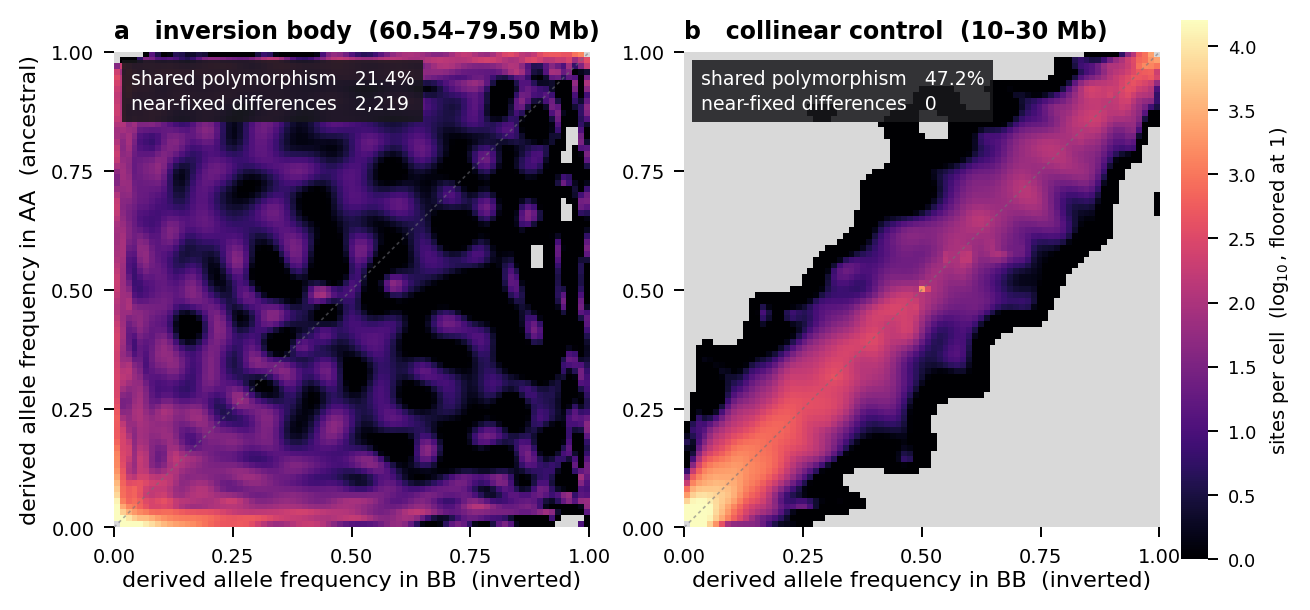
\includegraphics[width=.9\linewidth]{figS5_joint_sfs.png}
  \caption{\textbf{Joint two-dimensional site-frequency spectrum} of derived-allele frequency in the
    AA (ancestral) versus BB (inverted) arrangement. Each cell is a count of sites (colour, $\log_{10}$).
    In the inversion body (a) density spreads off the diagonal and into the corners, with variants common in one arrangement and absent in the other, i.e.\ near-fixed differences (2{,}219 sites; 21\% shared polymorphism), the direct signature of the recombination barrier. In the collinear control (b) the
    density collapses onto the diagonal (0 near-fixed differences; 47\% shared), as expected for freely
    recombining, exchangeable sequence. [Regeneration note. Drop interpolation, floor counts at 1, and mask empty cells to a distinct colour.]}
  \label{sfig:jsfs}
\end{figure}

\begin{figure}[h]\centering
  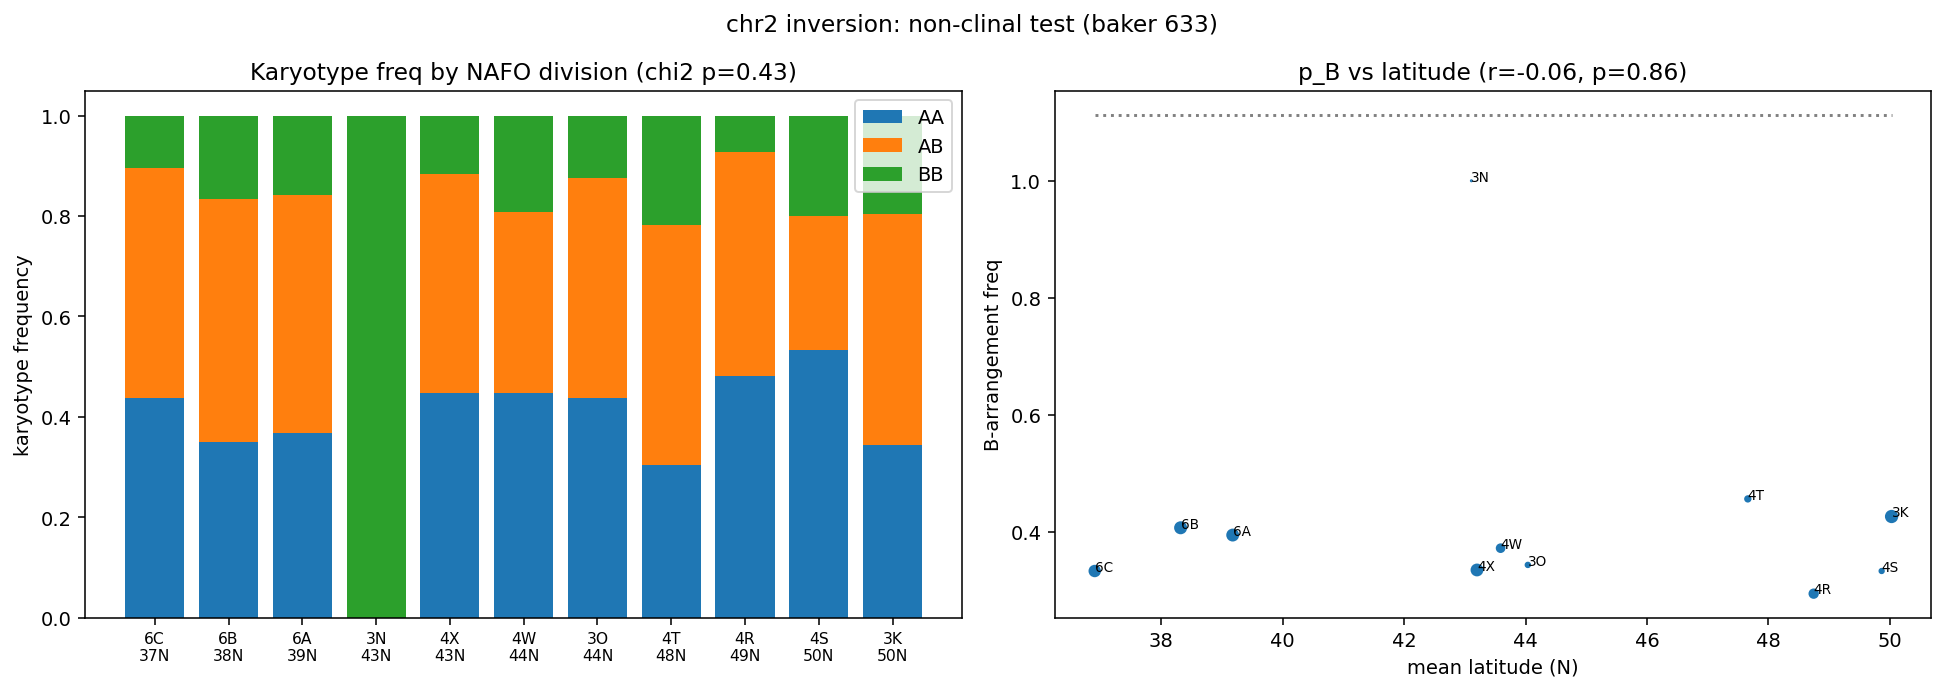
\includegraphics[width=.7\linewidth]{figS6_cline.png}
  \caption{\textbf{The inversion is non-clinal.} Inverted-arrangement frequency across NAFO sampling
    divisions shows no latitudinal trend (see \cref{stab:geo}); geographic $\Fst\approx0$, and the three
    karyotypes co-occur throughout the range.}
  \label{sfig:cline}
\end{figure}

\begin{figure}[h]\centering
  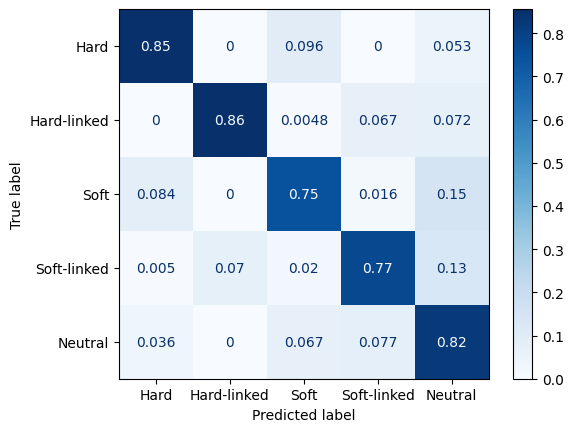
\includegraphics[width=.6\linewidth]{figS7_confusion.png}
  \caption{\textbf{Sweep-classifier confusion matrix} (five-class diploSHIC, full-SFS model; 81\% overall accuracy). Recall is 0.85 for hard, 0.86 for linked-hard, 0.82 for neutral, 0.75 for soft and 0.77 for linked-soft sweeps.}
  \label{sfig:confusion}
\end{figure}

\begin{figure}[h]\centering
  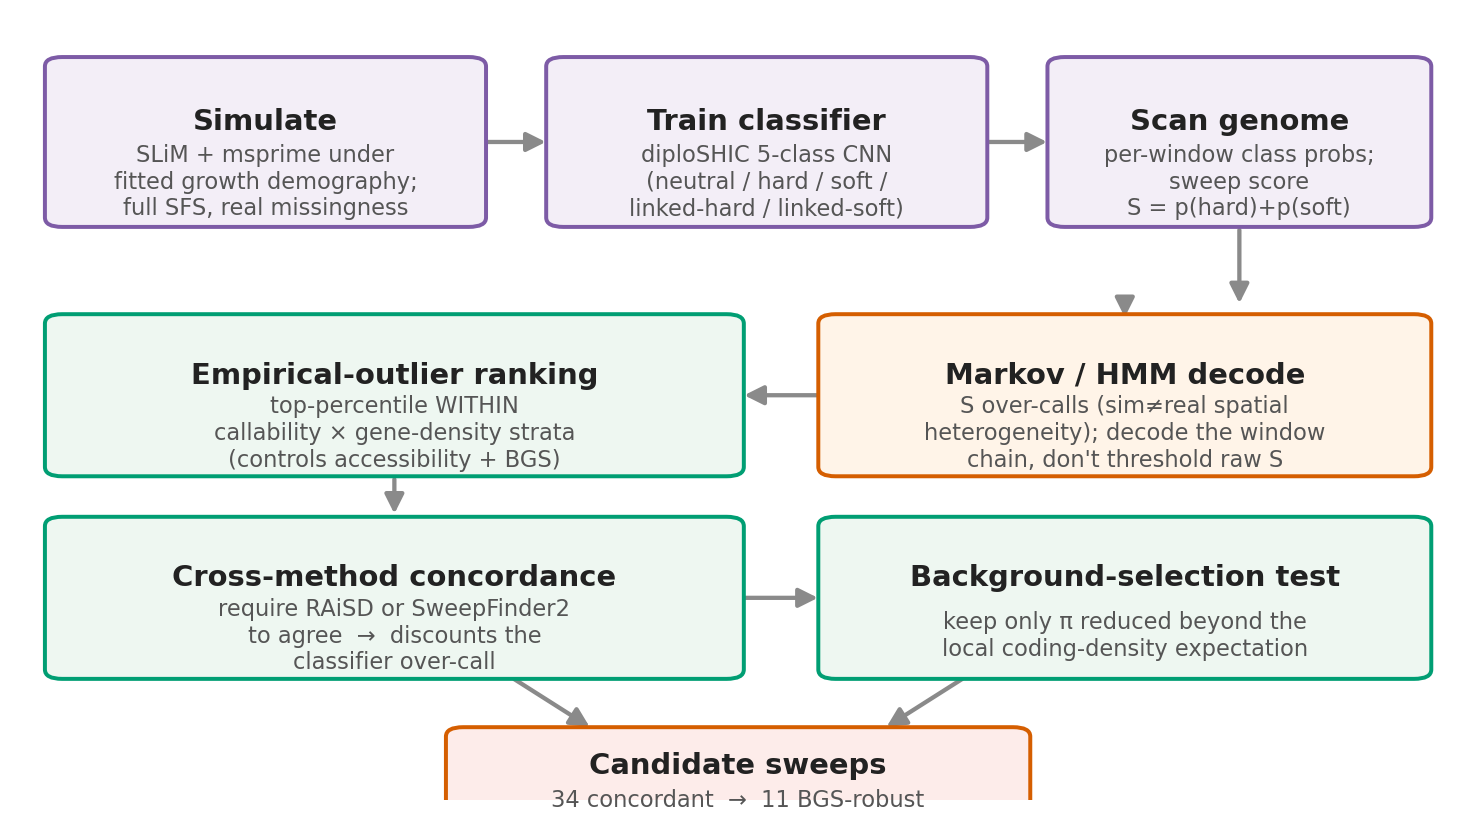
\includegraphics[width=.92\linewidth]{figS8_pipeline.png}
  \caption{\textbf{The selective-sweep scan pipeline.} Simulate (SLiM + msprime under the fitted growth
    demography) $\to$ diploSHIC five-class classifier $\to$ Markov/HMM decode $\to$ stratified
    empirical-outlier ranking (within callability $\times$ gene-density strata) + cross-method concordance
    (RAiSD, SweepFinder2) + background-selection filter $\to$ candidate sweeps.}
  \label{sfig:pipeline}
\end{figure}

\begin{figure}[h]\centering
  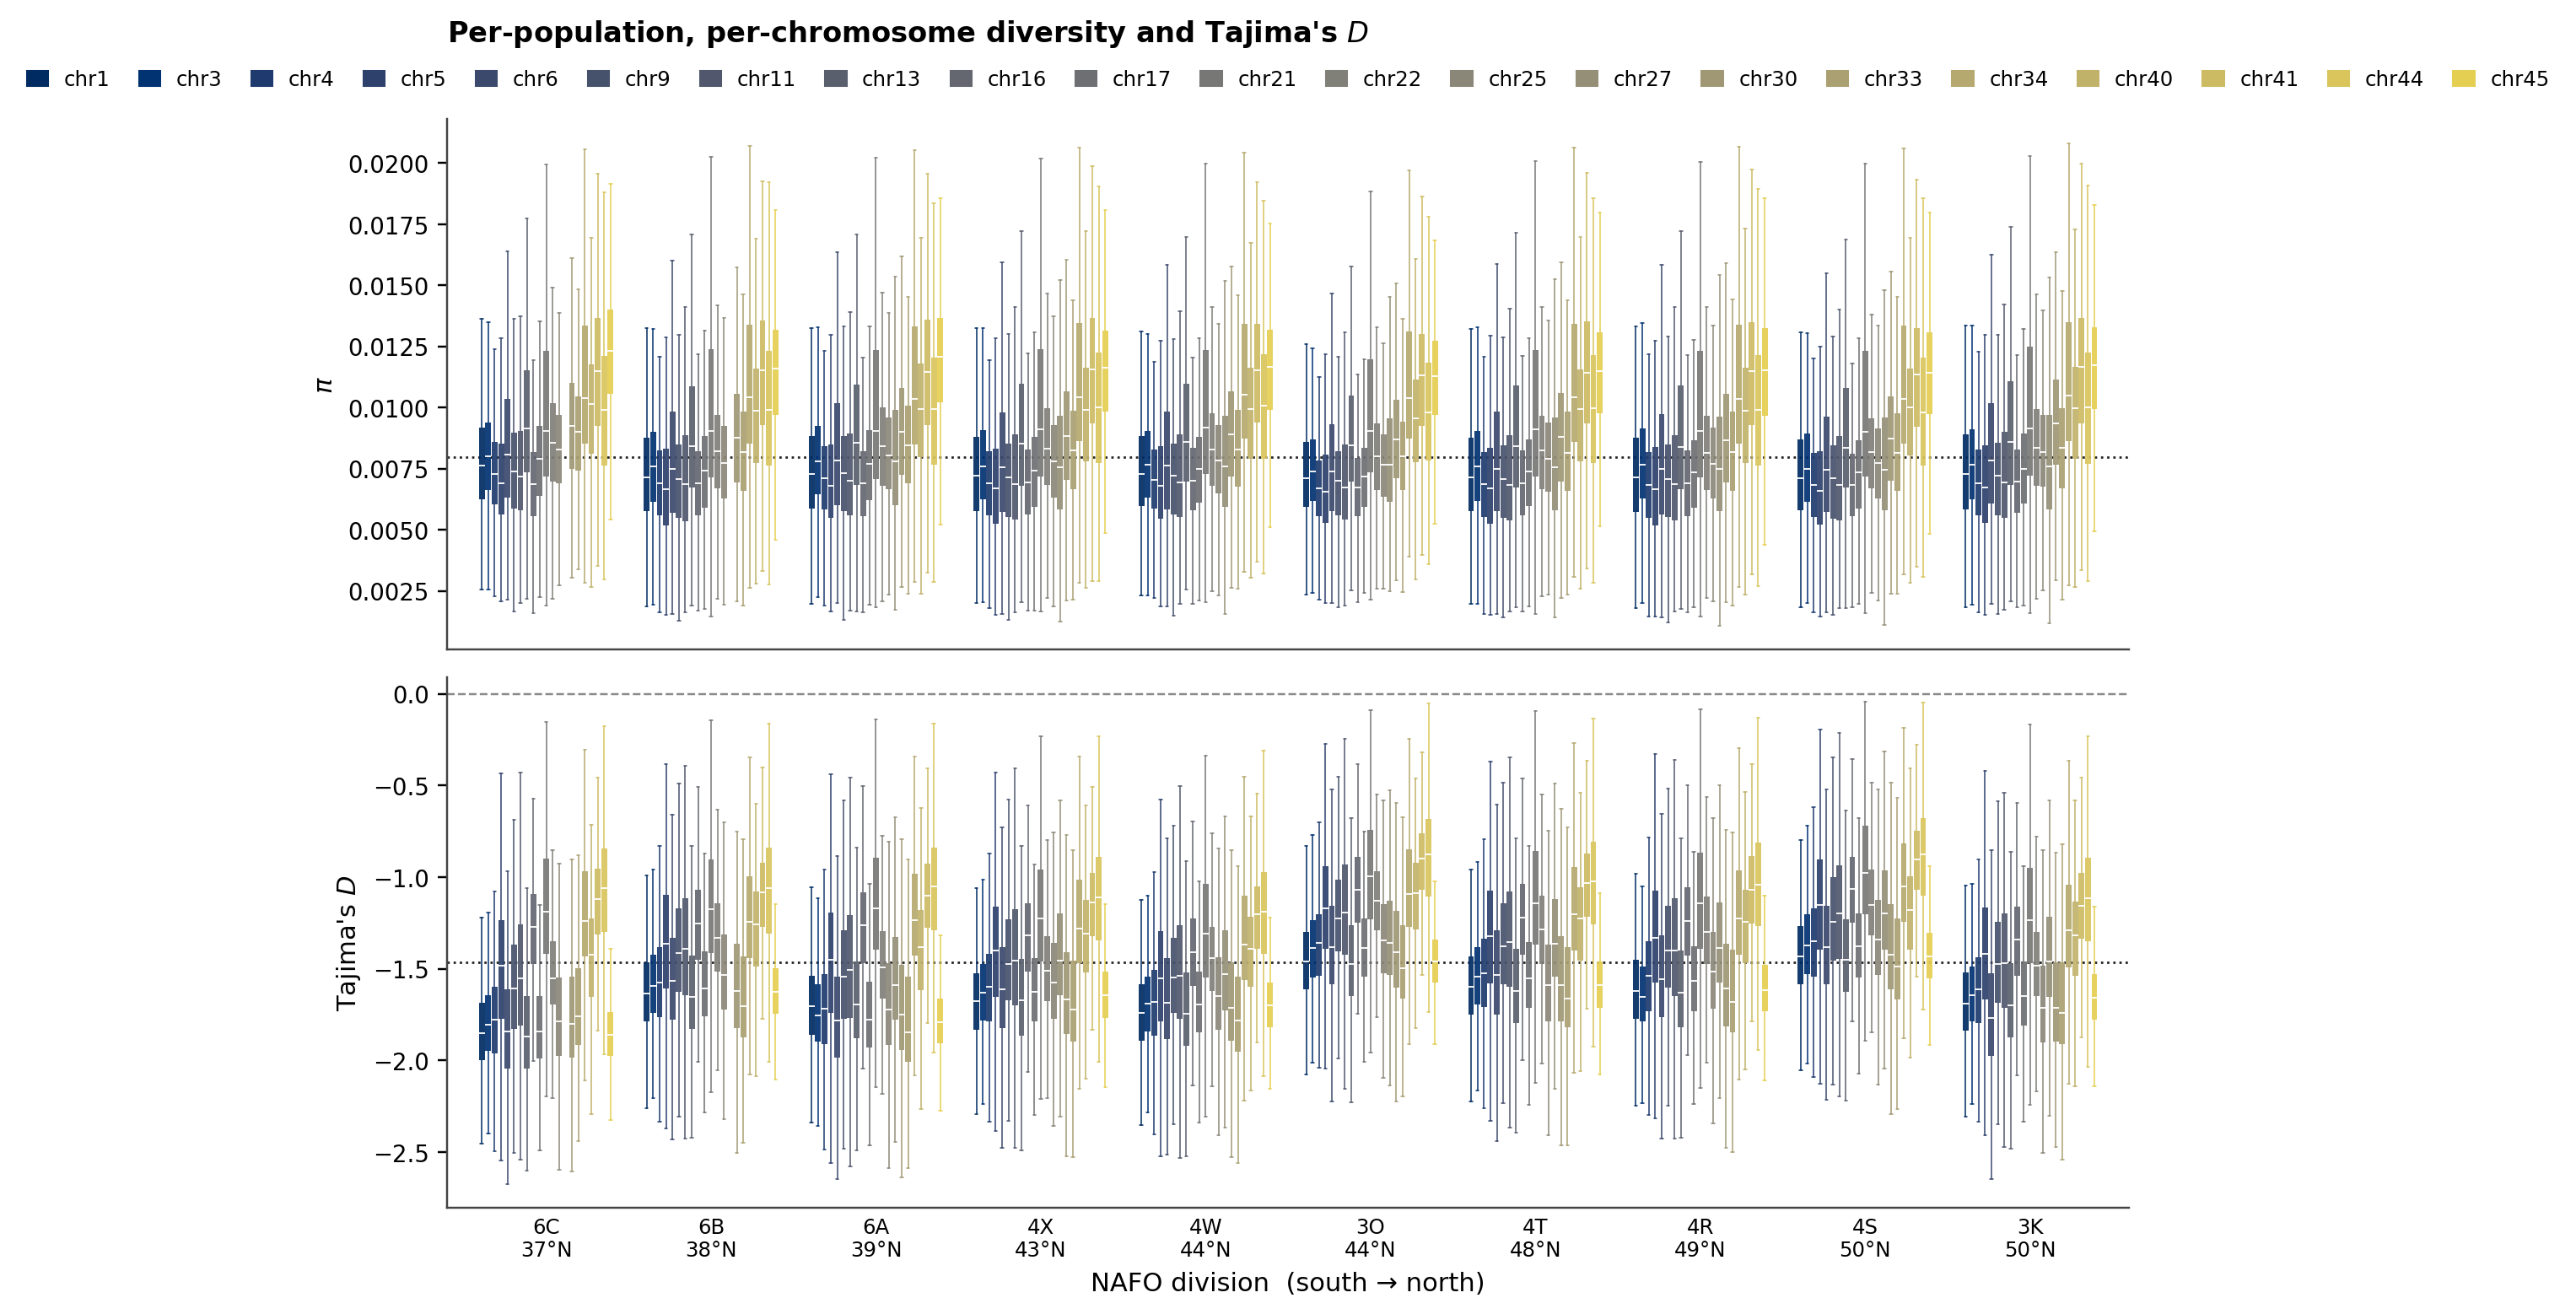
\includegraphics[width=\linewidth]{figS9_diversity_boxplots.png}
  \caption{\textbf{Per-chromosome diversity.} Distribution of nucleotide diversity $\pi$ (top) and Tajima's
    $D$ (bottom) across 50~kb windows, one box per chromosome (pooled over the ten NAFO divisions; all 46 chromosomes, 45 autosomes plus chrZ). Diversity is uniform and $D$ is strongly negative genome-wide, the signature of
    expansion. Two chromosomes stand apart. Chromosome~2 (the inversion; orange) carries an inflated upper
    tail of $\pi$ and more-negative $D$ from the segregating arrangements, and chrZ (blue; computed
    in the 330 hemizygous-informative males only, as females are Z-haploid) has reduced diversity
    ($\pi$ median 0.005 vs $\sim$0.008 autosomal, $\approx$0.63$\times$) as expected for a sex chromosome.}
  \label{sfig:divbox}
\end{figure}

\begin{figure}[h]\centering
  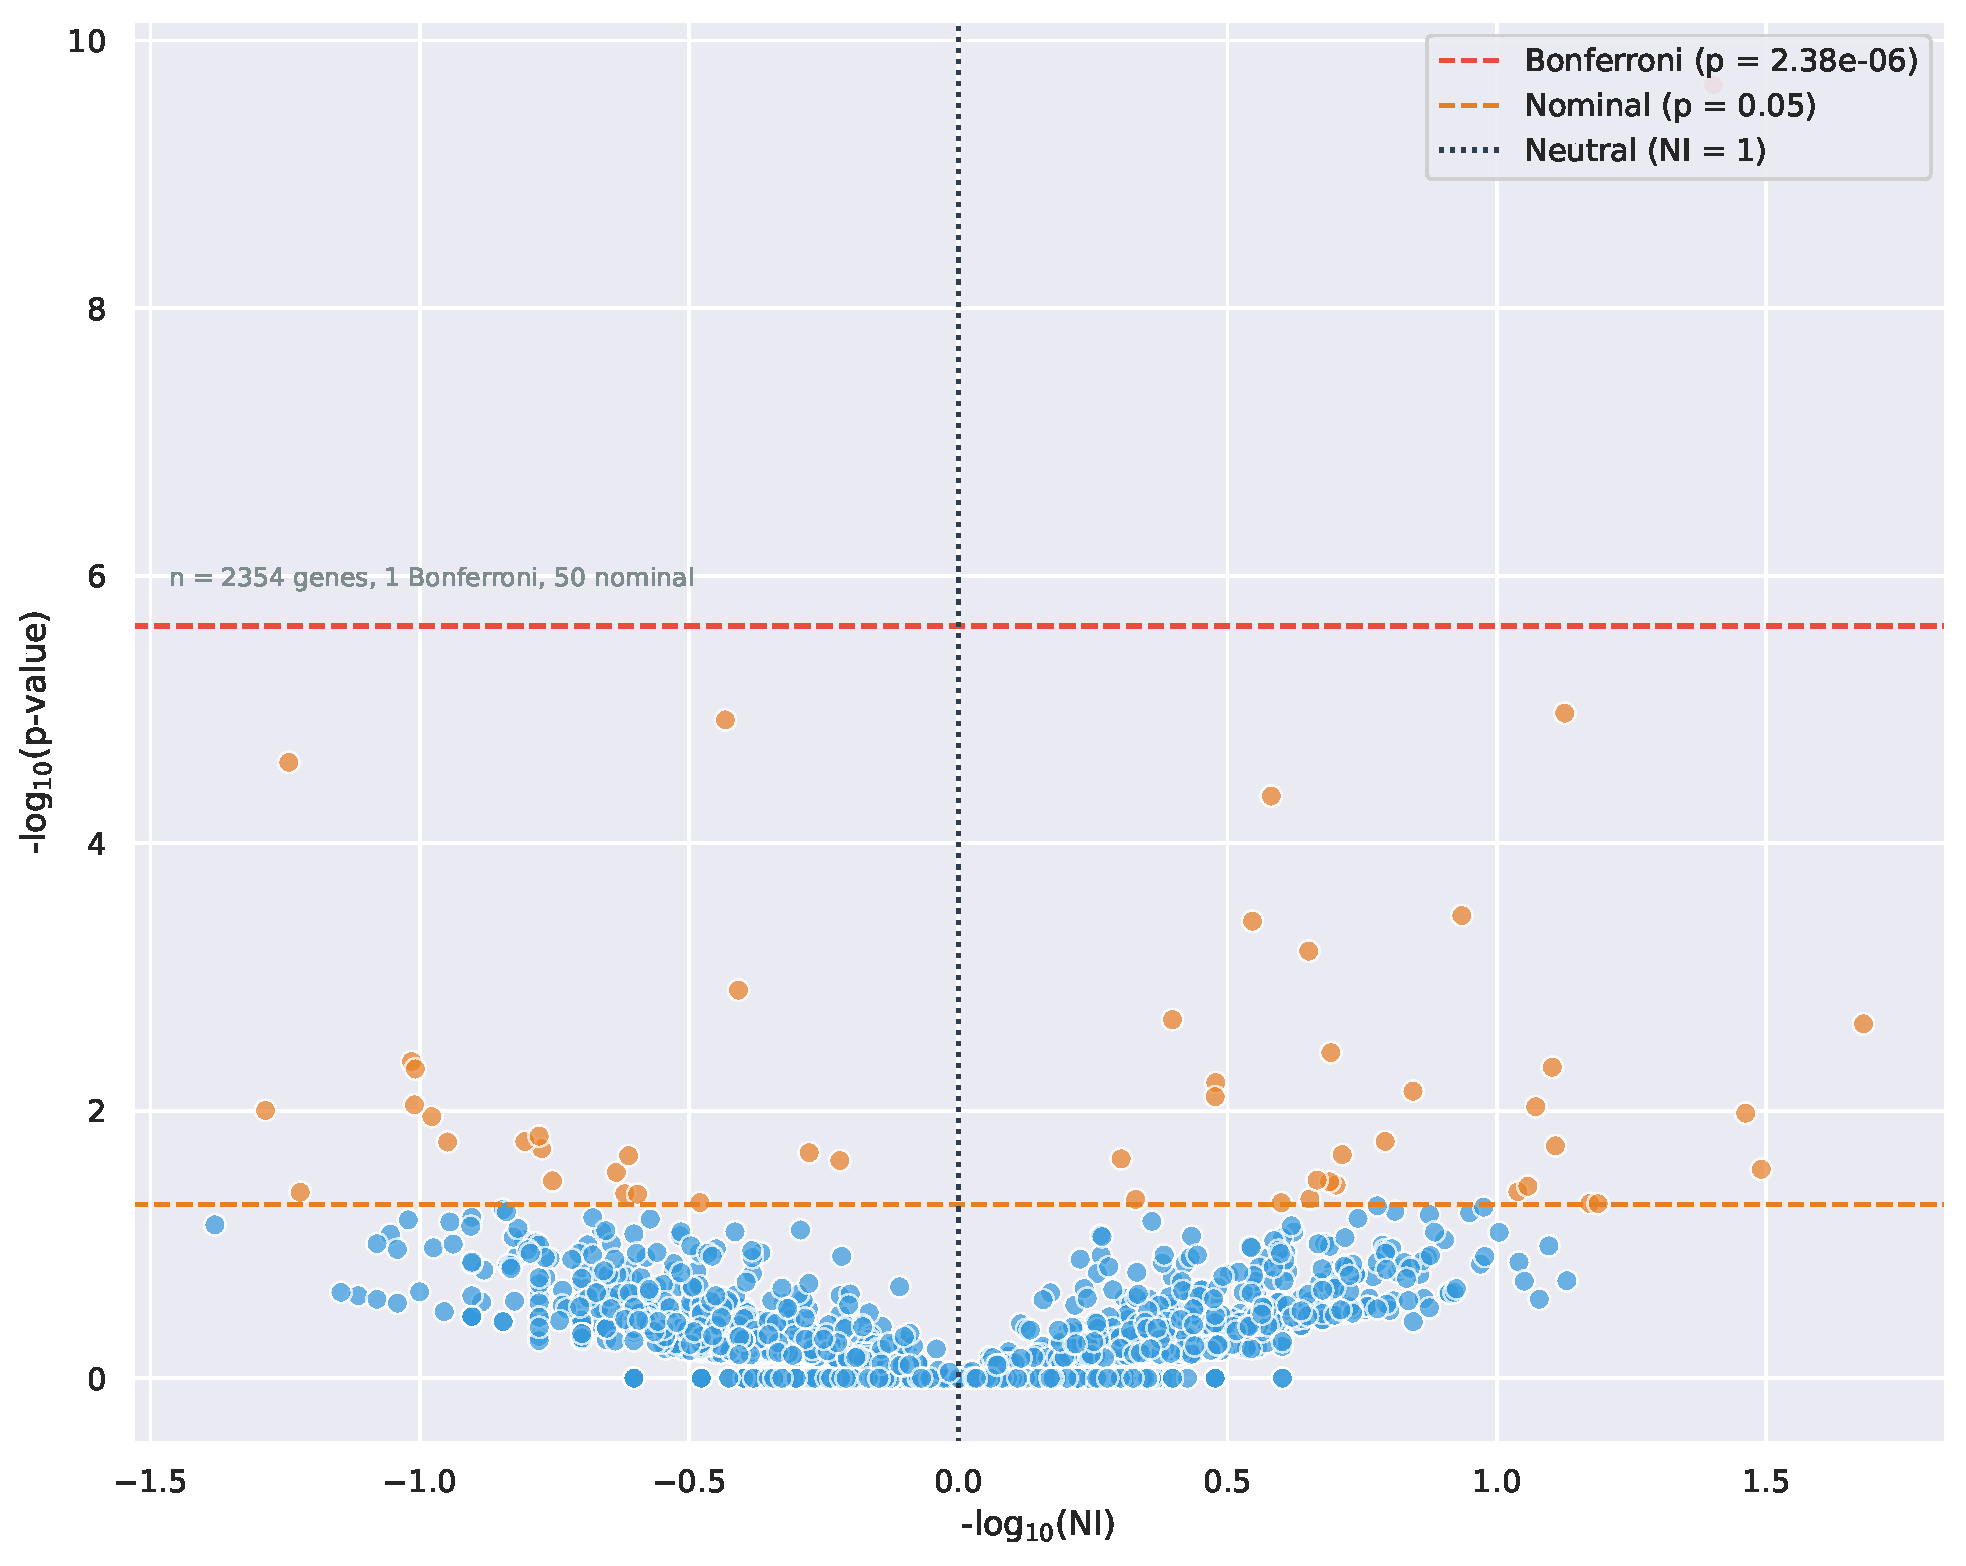
\includegraphics[width=.8\linewidth]{figS10_mkado.png}
  \caption{\textbf{Per-gene McDonald--Kreitman neutrality index} (mkado volcano plot, \coin{} outgroup).
    Each point is one gene, plotted as $-\log_{10}$ of its neutrality index NI\,$=(P_n/P_s)/(D_n/D_s)$ on the $x$-axis
    (right of the neutral NI\,$=1$ line $=$ adaptive, $\mathrm{NI}<1$; left $=$ excess non-synonymous
    polymorphism, $\mathrm{NI}>1$) against $-\log_{10}p$ on the $y$-axis. Dashed lines mark the nominal
    ($p=0.05$) and Bonferroni thresholds. Of $n=2{,}354$ testable genes, 50 are nominally significant and 1
    survives Bonferroni; the genome-wide asymptotic $\alpha=0.64$ resolves to few individual genes, as
    expected for a large-$N_e$ species where per-gene MK is underpowered.}
  \label{sfig:mkado}
\end{figure}

\begin{figure}[h]\centering
  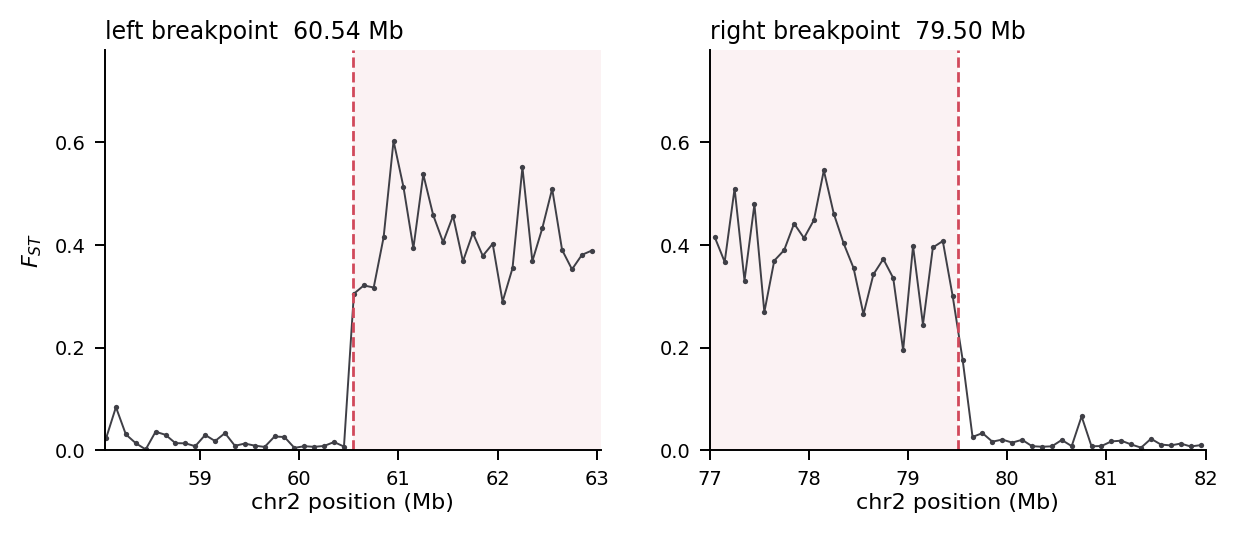
\includegraphics[width=.9\linewidth]{figS11_breakpoints.png}
  \caption{\textbf{Inversion breakpoints.} $\Fst$ across the left (60.54~Mb) and right (79.50~Mb) breakpoints, a step rather than a ramp.}
  \label{sfig:breakpoints}
\end{figure}

\begin{figure}[h]\centering
  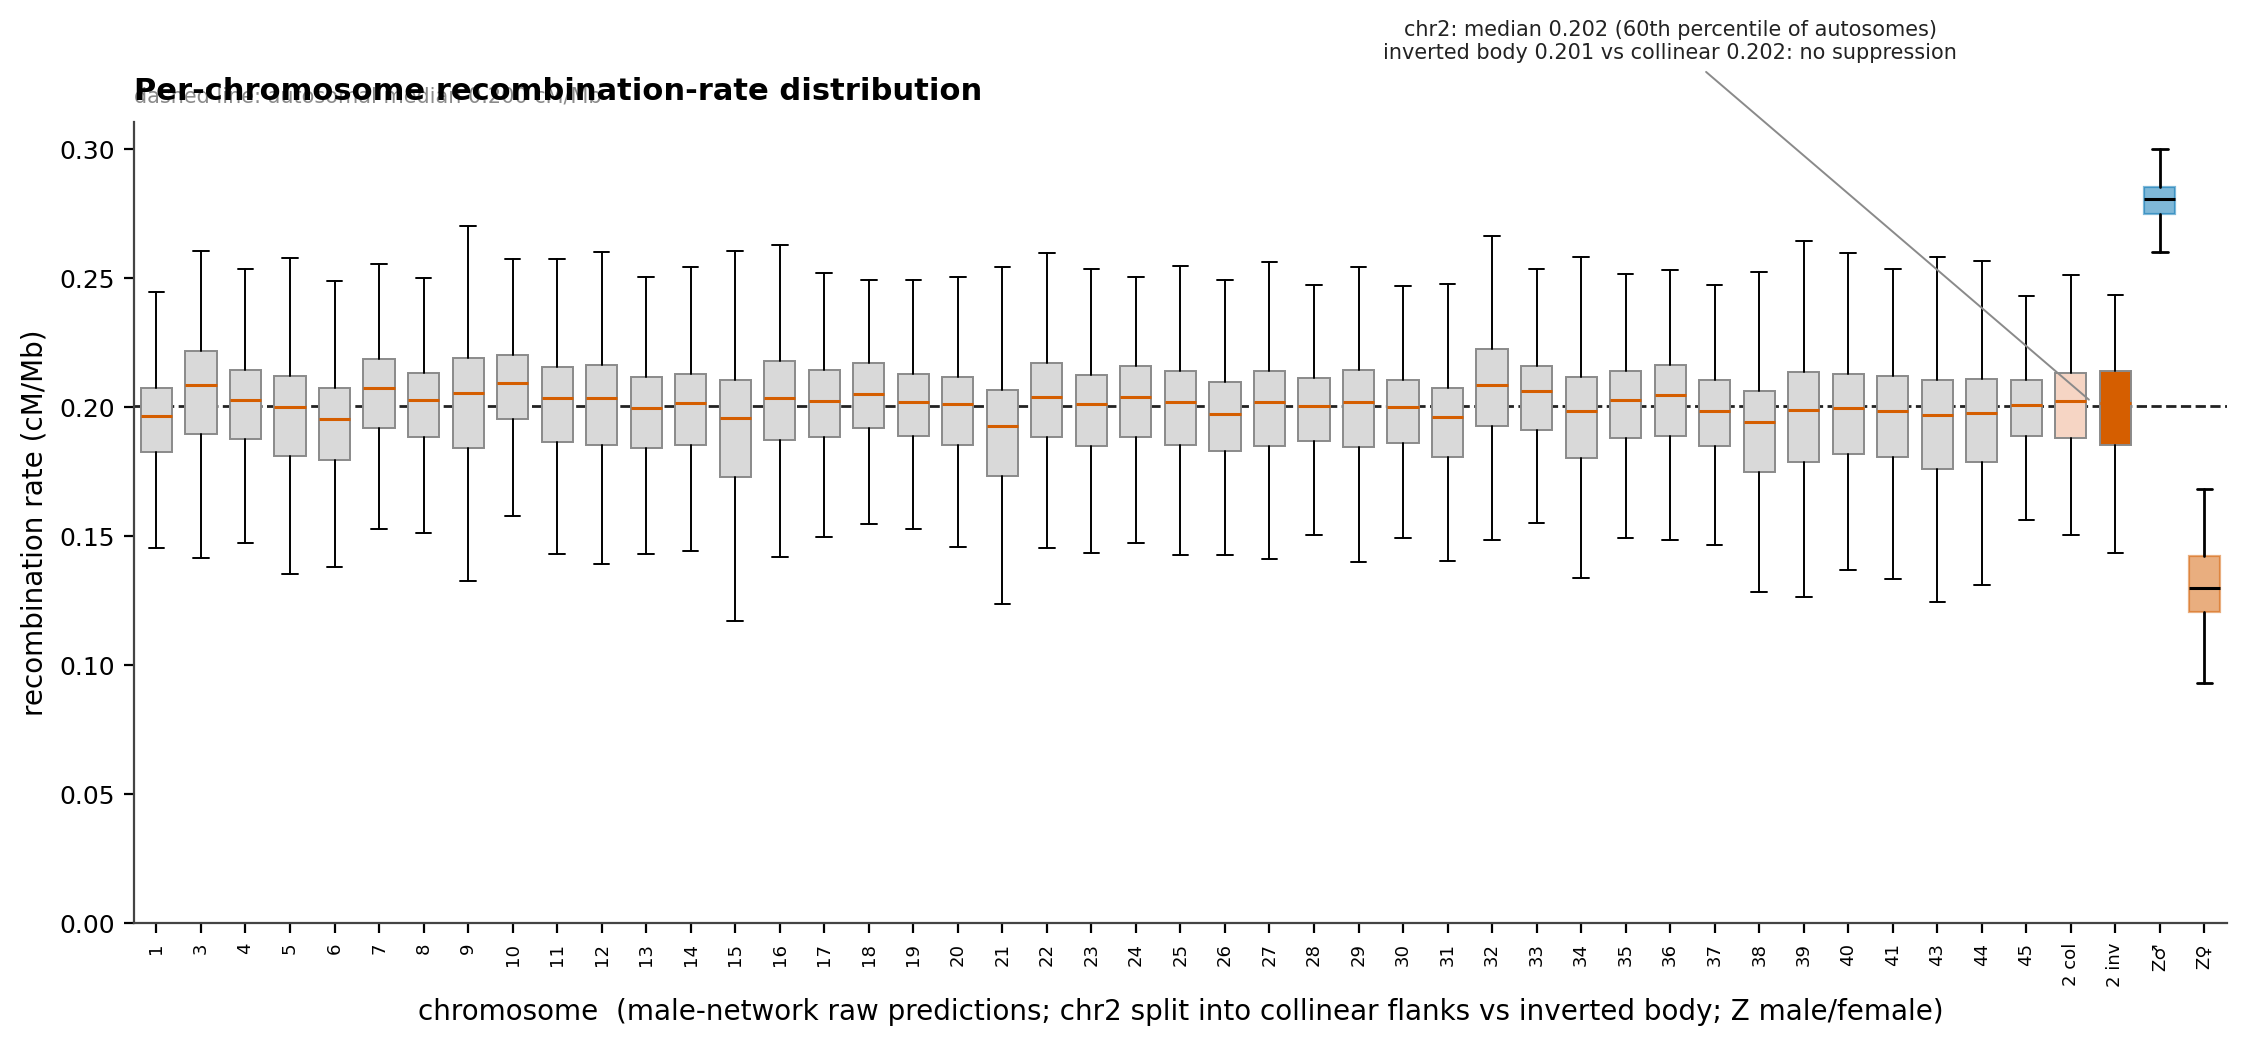
\includegraphics[width=.9\linewidth]{figS12_recomb_boxplots.png}
  \caption{\textbf{Per-chromosome recombination-rate distribution} (ReLERNN). All boxes are raw ReLERNN predictions from a single network so that chromosomes are compared on the same footing. They cover the 43 scanned autosomes, chromosome~2 restricted to its collinear sequence (2$^{*}$), and the Z. Collinear chromosome~2 recombines at an ordinary autosomal rate (median 0.202 vs 0.200~cM/Mb genome-wide, the 60th percentile of per-chromosome medians). The inverted body (60.54--79.50~Mb) is not shown, because this window-scale map, estimated from all karyotypes together, cannot resolve a barrier that acts only between arrangements. That barrier is shown directly by the linkage-disequilibrium block spanning the inversion (Supplementary Fig.~S4).}
  \label{sfig:recombbox}
\end{figure}

\begin{figure}[h]\centering
  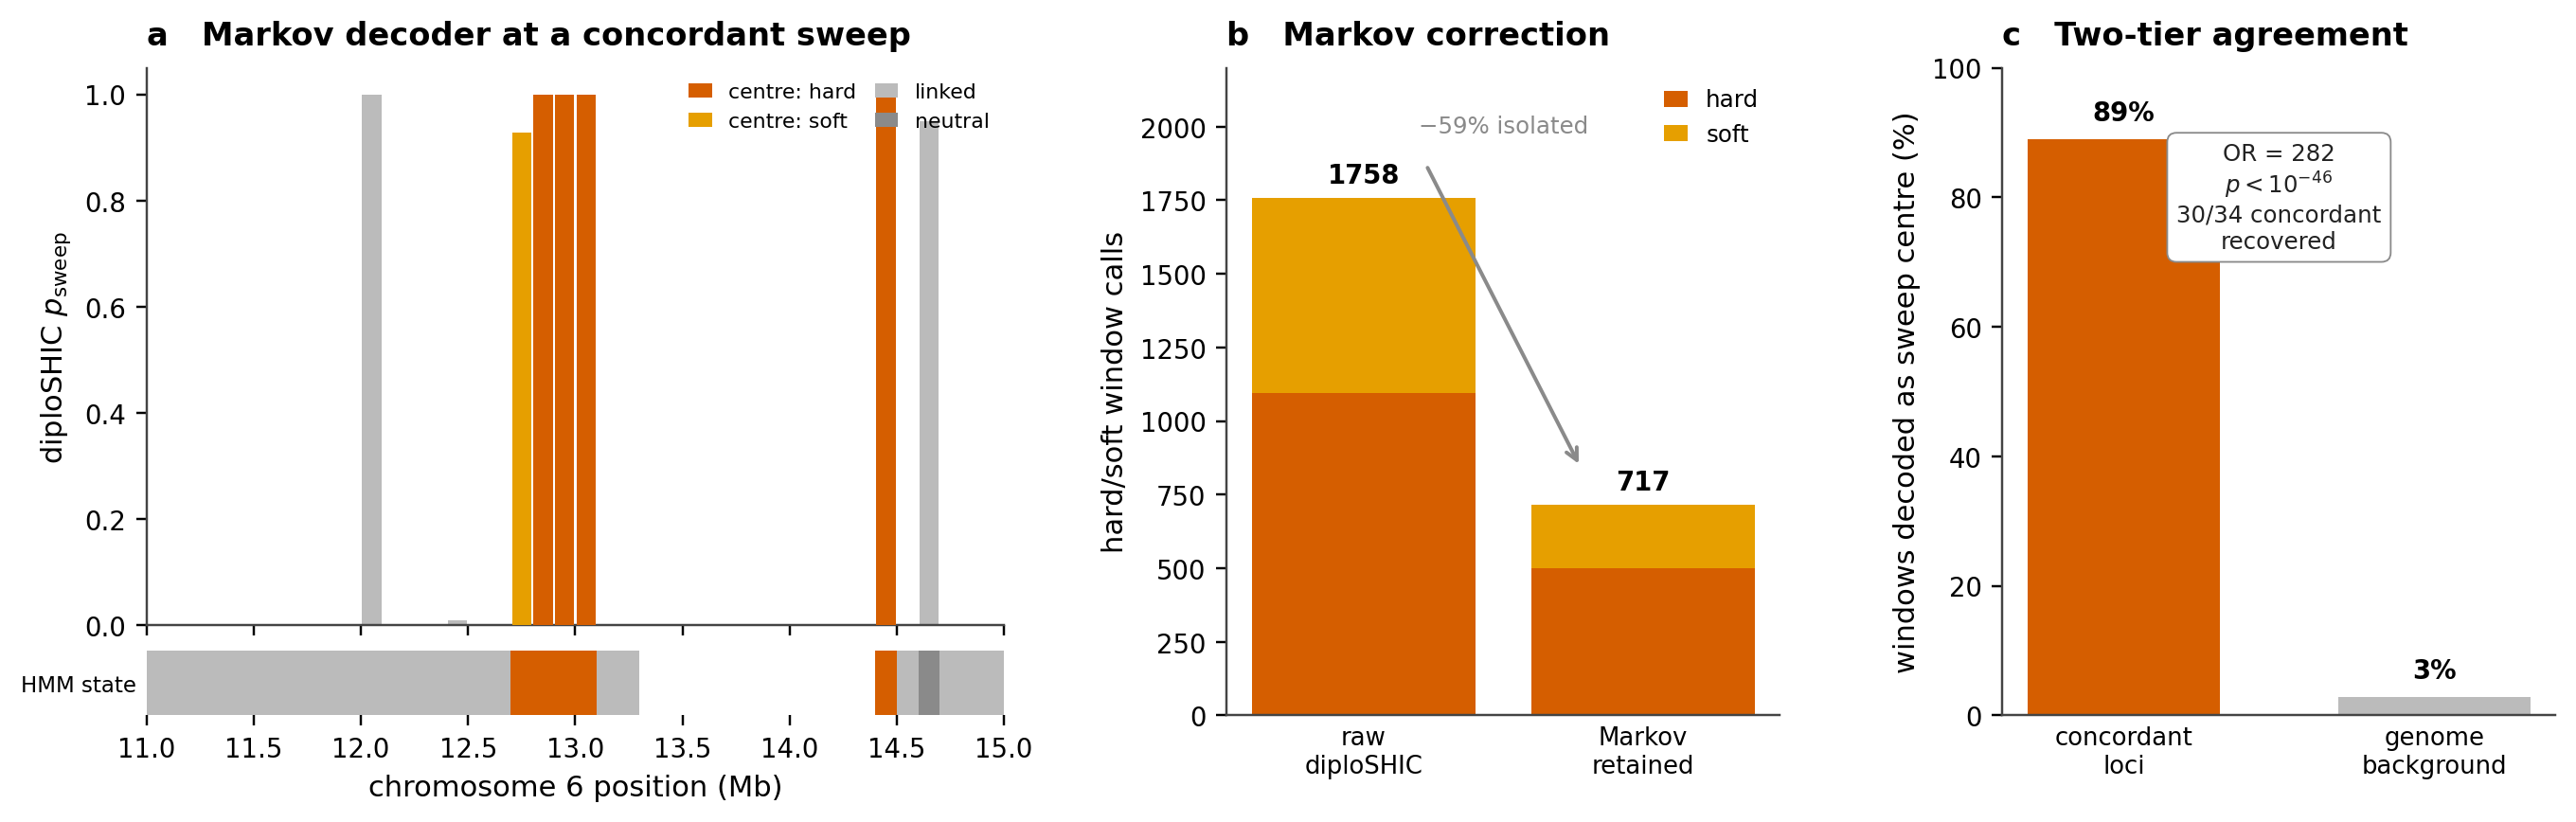
\includegraphics[width=\linewidth]{figS13_markov.png}
  \caption{\textbf{Recombination-aware Markov decoder for the Tier-1 sweep calls.} A hidden Markov model over
    the per-100~kb-window diploSHIC classification (emissions $=$ prior-corrected class posteriors; dwell
    lengths from the $\sim$400~kb sweep footprint scaled by the ReLERNN map; design-informed, not
    simulation-calibrated). \textbf{(a)}~The decoder at a representative concordant sweep (chromosome~35, \textit{ZEB2}), showing the sweep posterior $p_\mathrm{hard}+p_\mathrm{soft}$ per window and the Viterbi state track
    (neutral / linked / centre); it localises the centre inside the linked envelope and overrides spatially
    isolated high-posterior windows (e.g.\ near 38.35~Mb). \textbf{(b)}~Markov correction reduces the raw
    hard/soft calls from 1{,}651 to 677 spatially coherent calls ($-59\%$). \textbf{(c)}~88\% of windows at
    the Tier-2 cross-method-concordant loci are decoded as sweep centres versus 2.9\% genome-wide (odds
    ratio 242, $p<10^{-30}$; 21 of 24 concordant regions recovered).}
  \label{sfig:markov}
\end{figure}

\begin{figure}[h]\centering
  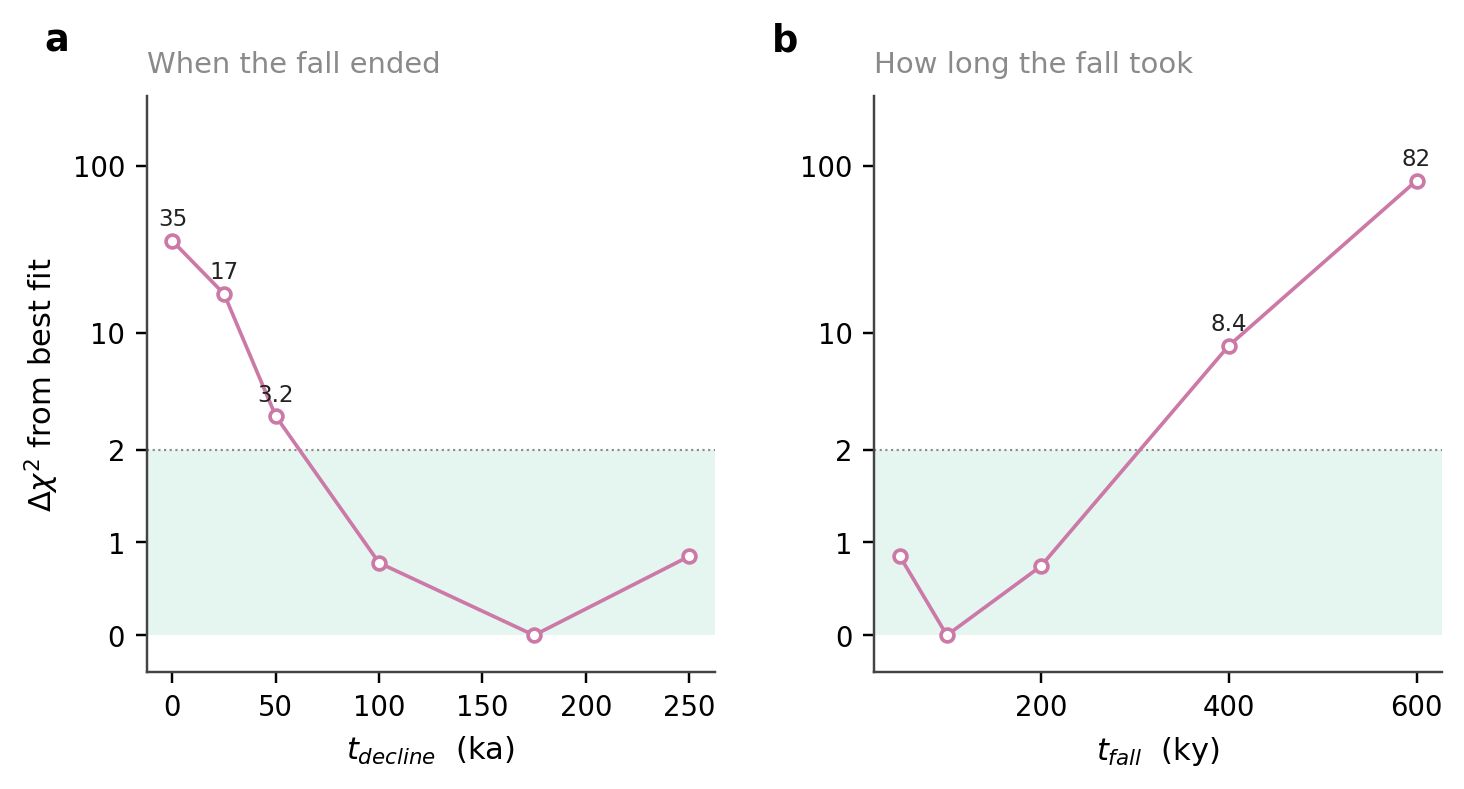
\includegraphics[width=.85\linewidth]{figS14_inversion_profiles.png}
  \caption{\textbf{Profile-likelihood bounds on the chromosome-2 inversion's decline}
    (main-text Fig.~4). $\Delta\chi^2$ from the best fit while profiling (a)~$t_\mathrm{decline}$, when
    the fall ended, and (b)~$t_\mathrm{fall}$, how long it took; the shaded band is $\Delta\chi^2<2$
    (not excluded). The fall ended $\sim$50--200~ka and took $\sim$50--200~ky.}
  \label{sfig:profiles}
\end{figure}

\begin{figure}[h]\centering
  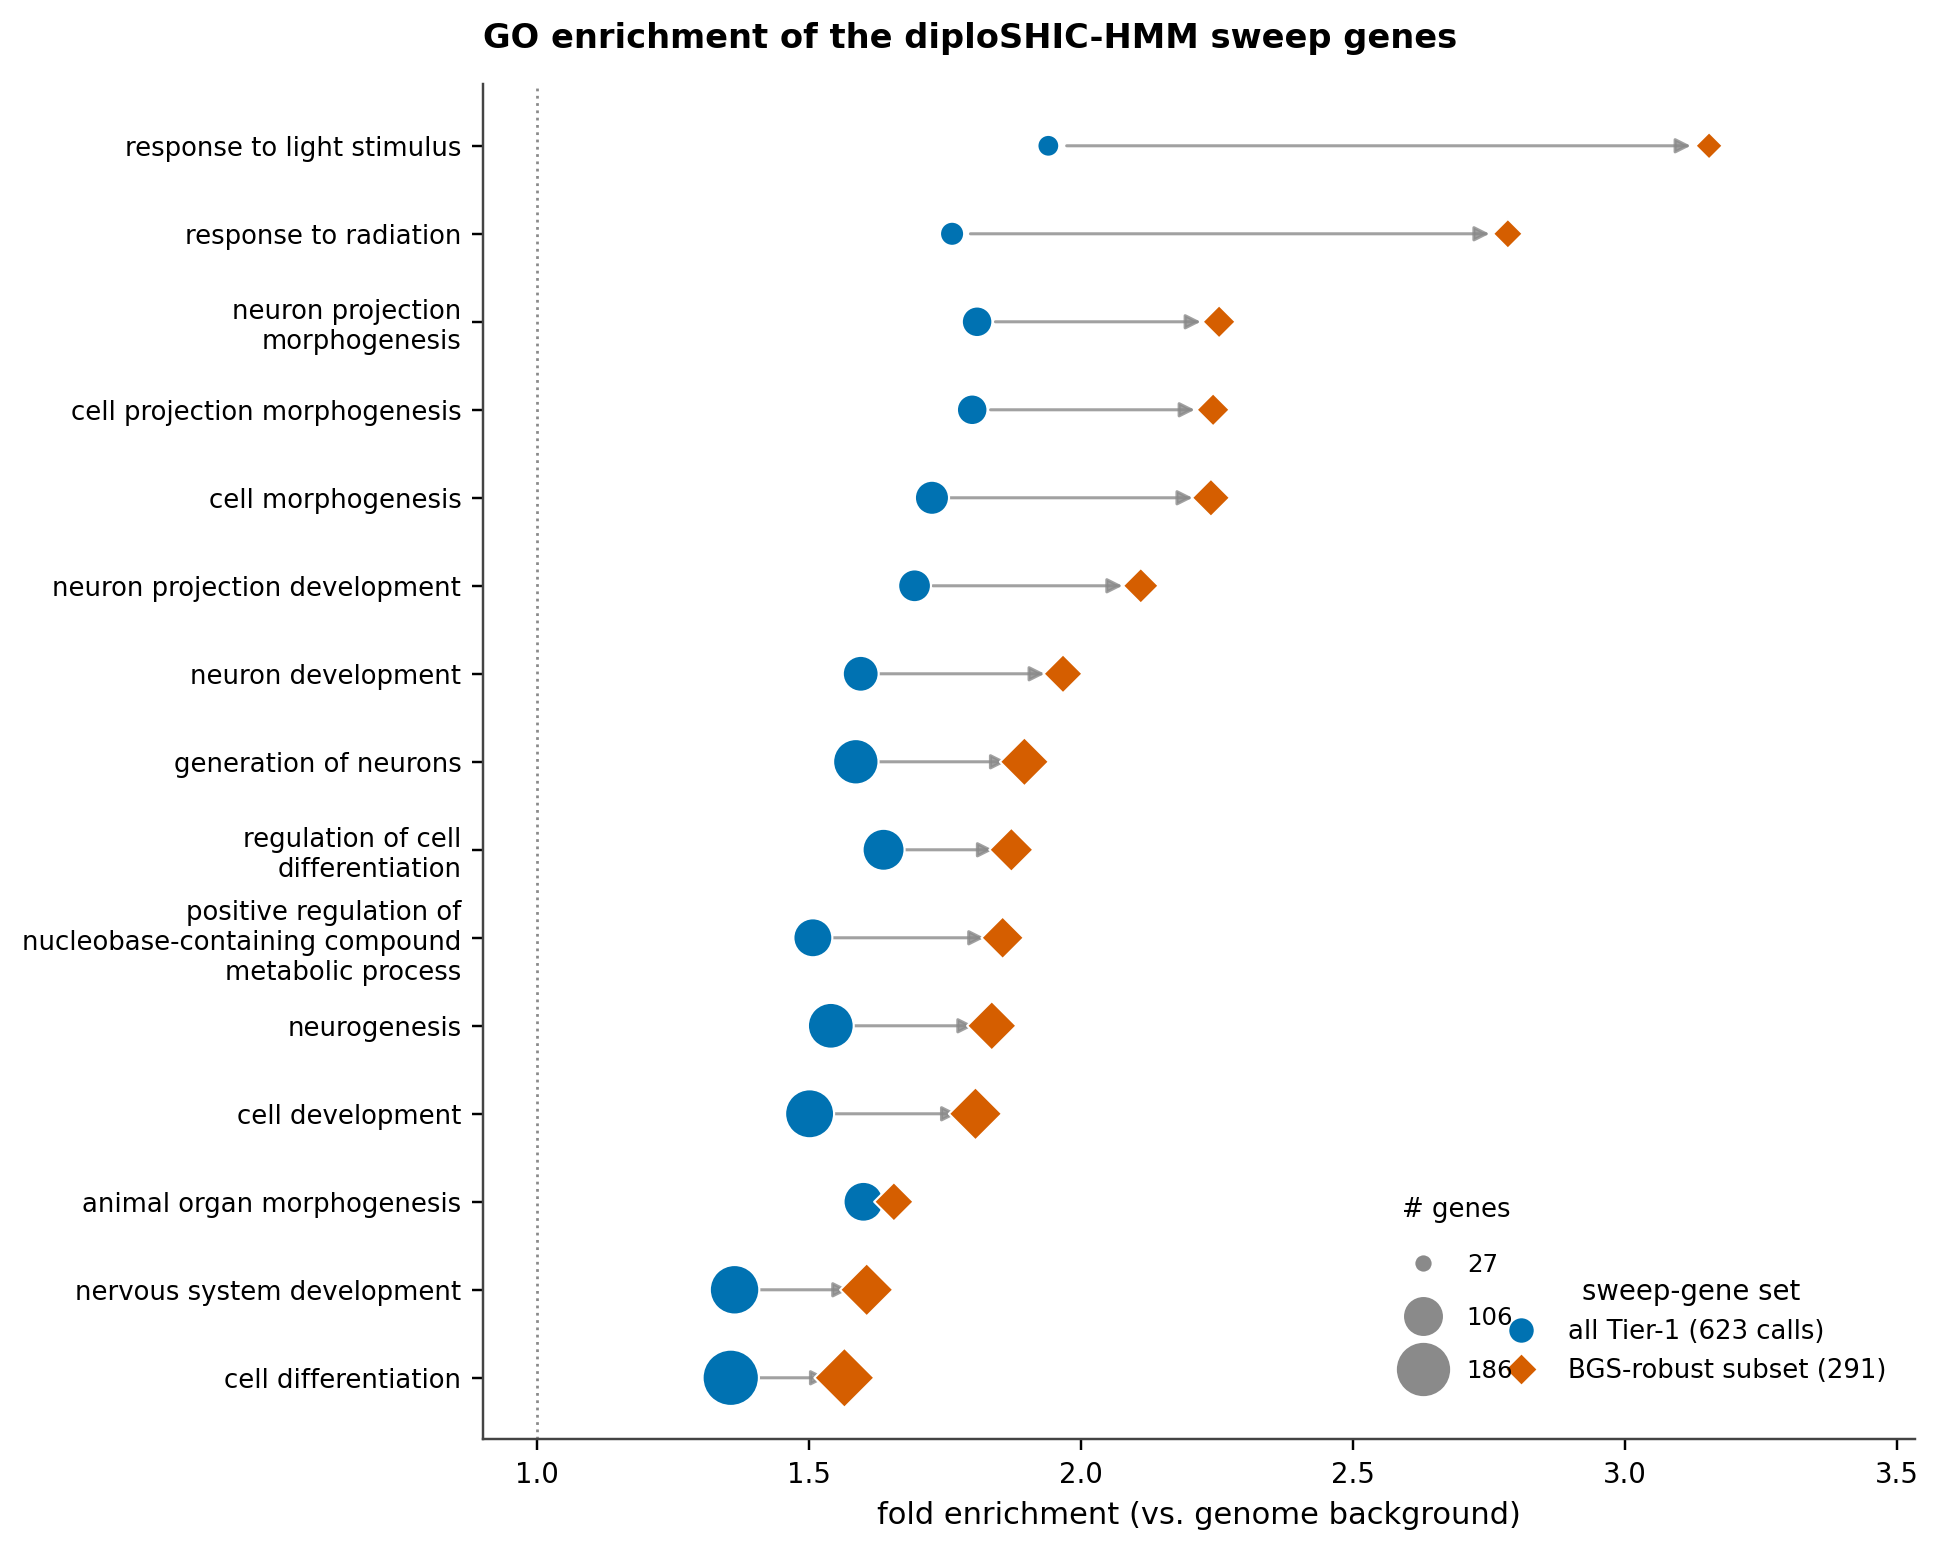
\includegraphics[width=.9\linewidth]{figS15_gsea.png}
  \caption{\textbf{GO enrichment of the diploSHIC-HMM sweep genes} (biological process; terms significant at
    FDR$<$0.05 in both sets). In this paired dot plot each term is shown for the full Tier-1 set (blue circle; 623 calls) and for its background-selection-robust subset (orange diamond; 291 calls), with $x=$ fold
    enrichment and marker area $=$ number of sweep genes carrying the term. The grey arrow marks the shift between the two sets. The BGS screen consistently sharpens the enrichment (rightward), and most
    strongly for the light-response / photoreception terms (response to light stimulus $1.9\to3.1\times$;
    response to radiation $1.8\to2.8\times$). Two coherent themes dominate, neural development and photoreception, and both survive the background-selection filter (\cref{stab:goenrich};
    full per-set enrichment tables are provided with the source). The hard-sweep calls are a
    sub-classification recorded in the calls table, not a separate gene set.}
  \label{sfig:gsea}
\end{figure}

\begin{figure}[h]\centering
  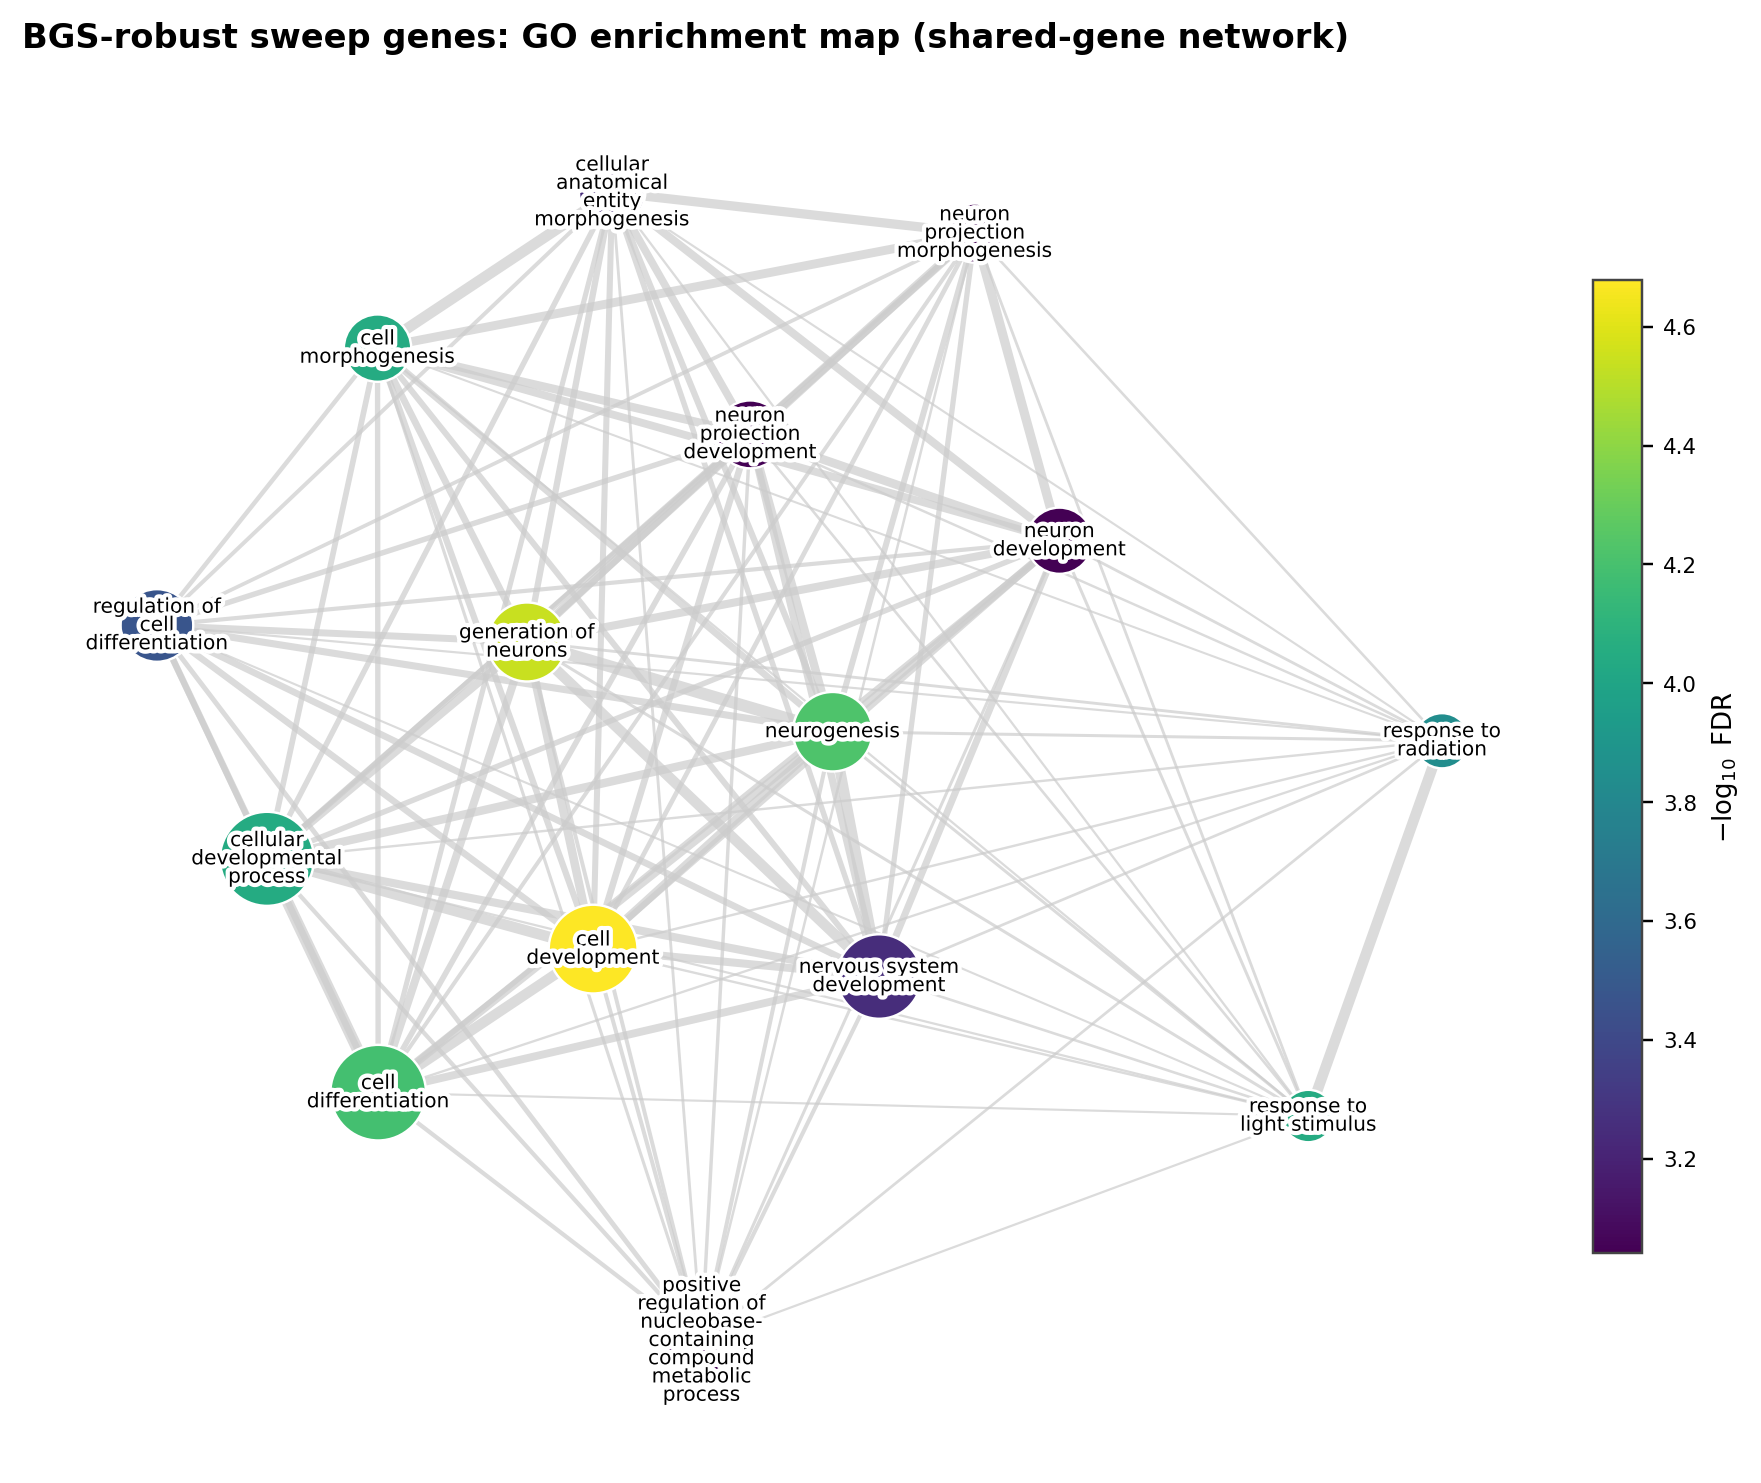
\includegraphics[width=.85\linewidth]{figS16_go_network.png}
  \caption{\textbf{GO enrichment map for the background-selection-robust sweep genes.} Built from the 291
    BGS-robust Tier-1 calls (the subset whose local diversity reduction exceeds the background-selection
    expectation; 227 GO-annotated genes). Nodes are enriched biological-process terms (size $=$ number of
    genes, colour $=-\log_{10}$ FDR); edges connect terms sharing genes (Jaccard $\geq0.15$). The terms form
    connected modules of neural development / cell morphogenesis and photoreception (response to
    light/radiation), the same two themes seen in the GSEA dot plot (\cref{sfig:gsea}).}
  \label{sfig:gonet}
\end{figure}

\begin{figure}[h]\centering
  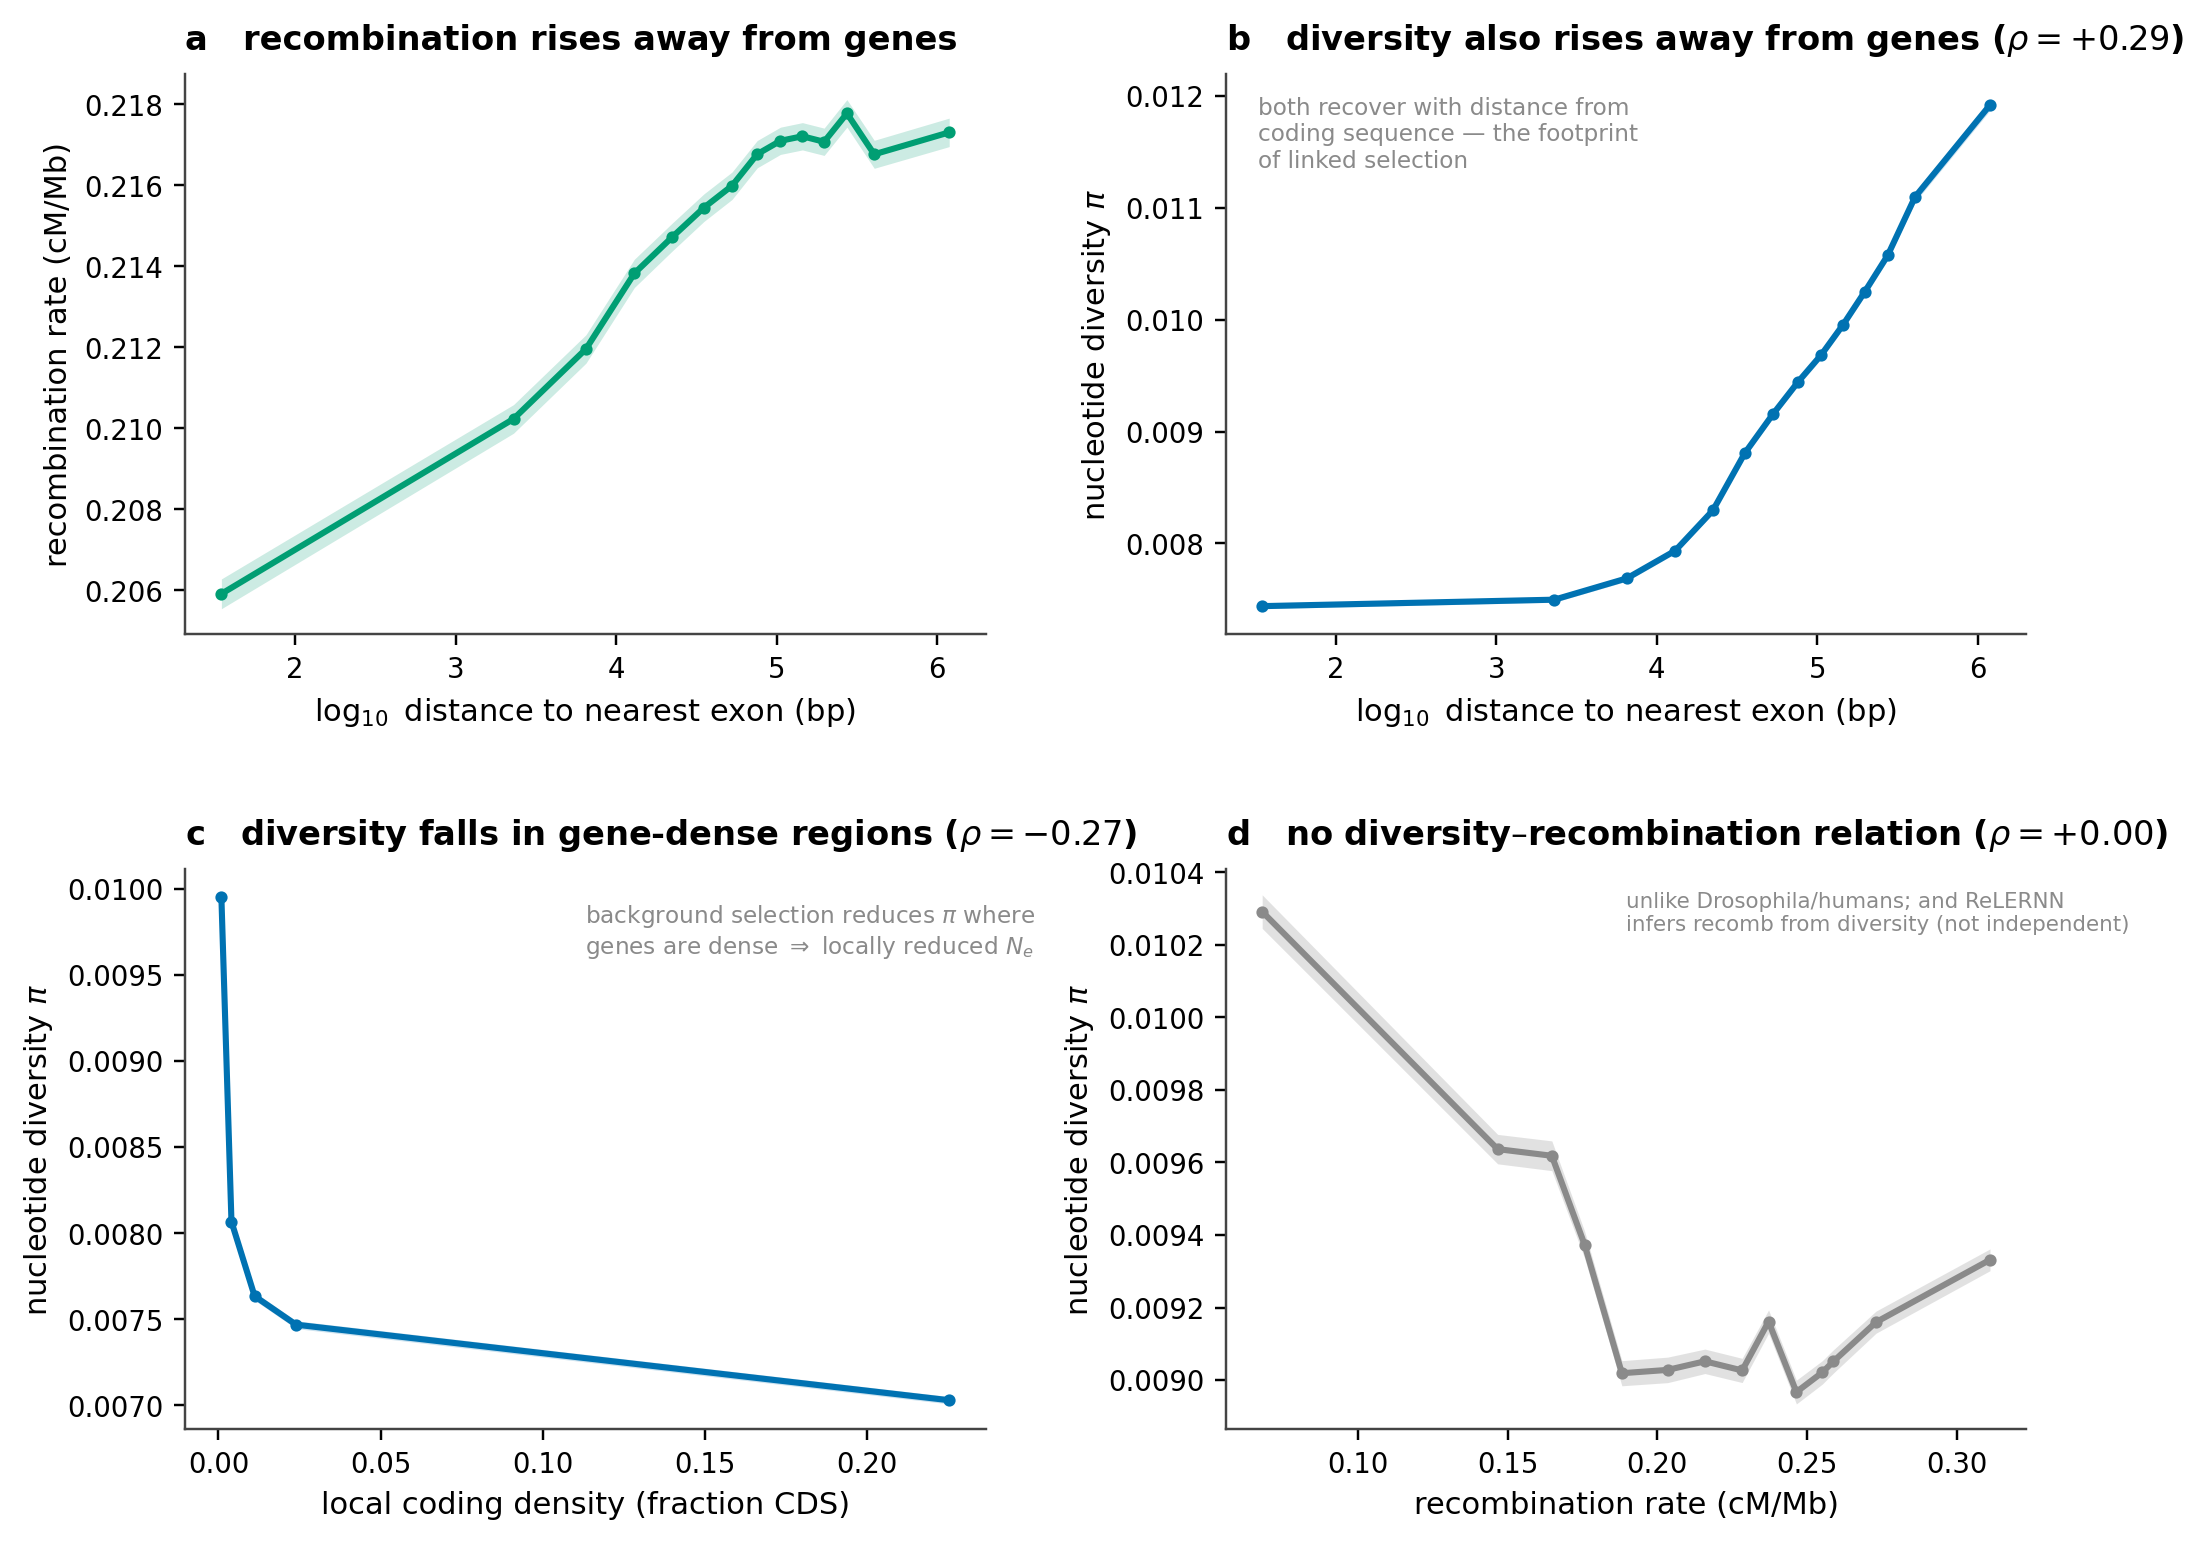
\includegraphics[width=\linewidth]{figS17_recomb_selection.png}
  \caption{\textbf{Recombination, gene proximity and the efficacy of selection.} Per-window statistics
    ($\sim$50~kb windows, autosomes). \textbf{(a)}~As a control, recombination rate is essentially flat across
    distance from the nearest exon (0.206$\to$0.217~cM/Mb near$\to$far, a $\sim$6\% range; Spearman
    $\rho=+0.05$, unchanged when $\pi$ is held fixed, partial $\rho=+0.06$), so recombination is agnostic to gene content, as it should be. \textbf{(b)}~Nucleotide diversity $\pi$, by contrast, rises steeply with
    distance from coding sequence ($\rho=+0.29$; +43\% near$\to$far), the footprint of linked selection.
    \textbf{(c)}~$\pi$ falls with local coding density ($\rho=-0.27$), as background selection reduces diversity where genes are dense, i.e.\ a locally reduced effective size, and it is
    gene-density-driven. Linked selection in \illex{} is thus structured by gene density and gene
    proximity rather than by the recombination-rate axis, which is nearly uniform genome-wide
    (0.2--0.24~cM/Mb; Supplementary Fig.~S22).}
  \label{sfig:recombsel}
\end{figure}

\begin{figure}[h]\centering
  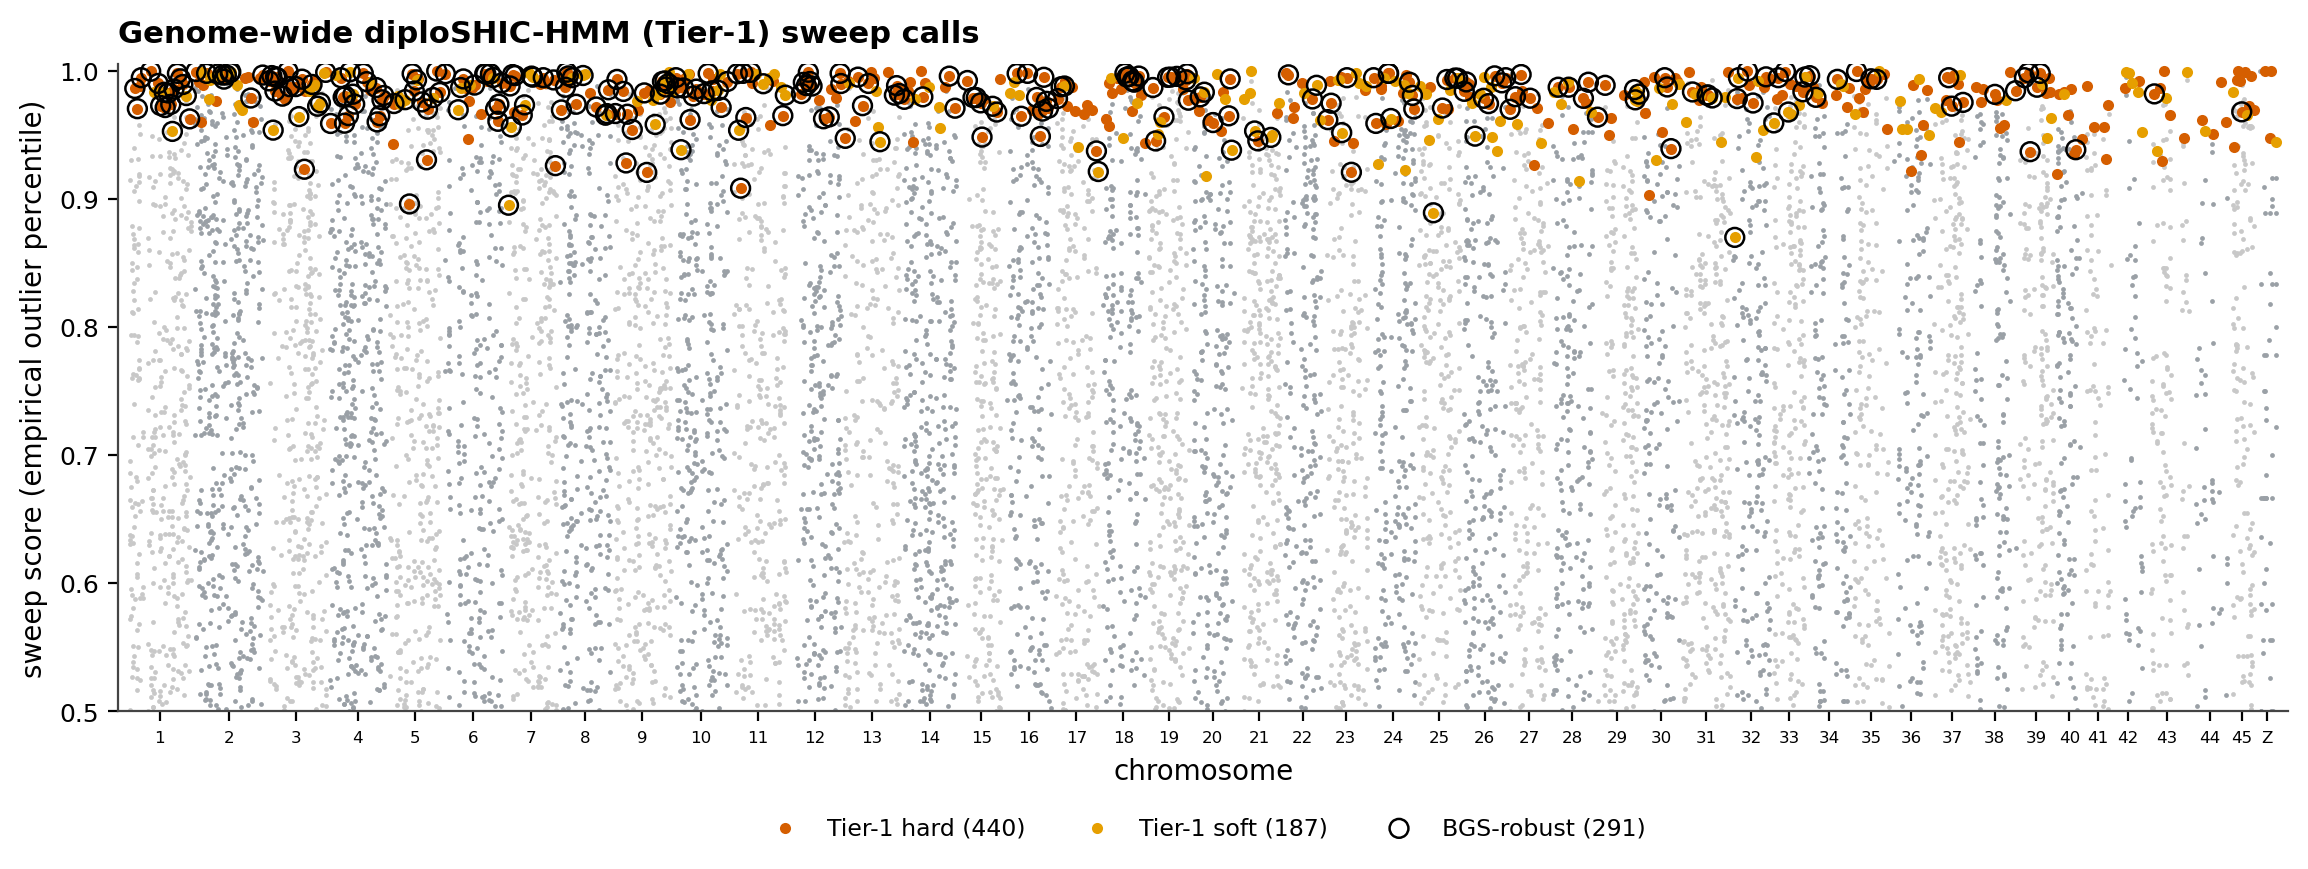
\includegraphics[width=\linewidth]{figS18_tier1_manhattan.png}
  \caption{\textbf{Genome-wide diploSHIC-HMM (Tier-1) sweep calls.} Per-100~kb-window empirical-outlier
    sweep score (rank within callability $\times$ coding-density strata) across all 45 autosomes plus the
    Z chromosome (627 calls total; 440 hard, 187 soft). The Markov-decoded Tier-1 calls are highlighted by
    class (hard, soft), and the background-selection-robust subset (\S\,BGS screen; 291 of the 623 autosomal calls) is ringed. The four chromosome-Z calls come from the male-only ($n{=}330$) diploSHIC scan and are
    diploSHIC-only (RAiSD/SweepFinder2 do not cover the Z). The calls are distributed across the genome with
    no single dominant locus.}
  \label{sfig:t1man}
\end{figure}

\begin{figure}[h]\centering
  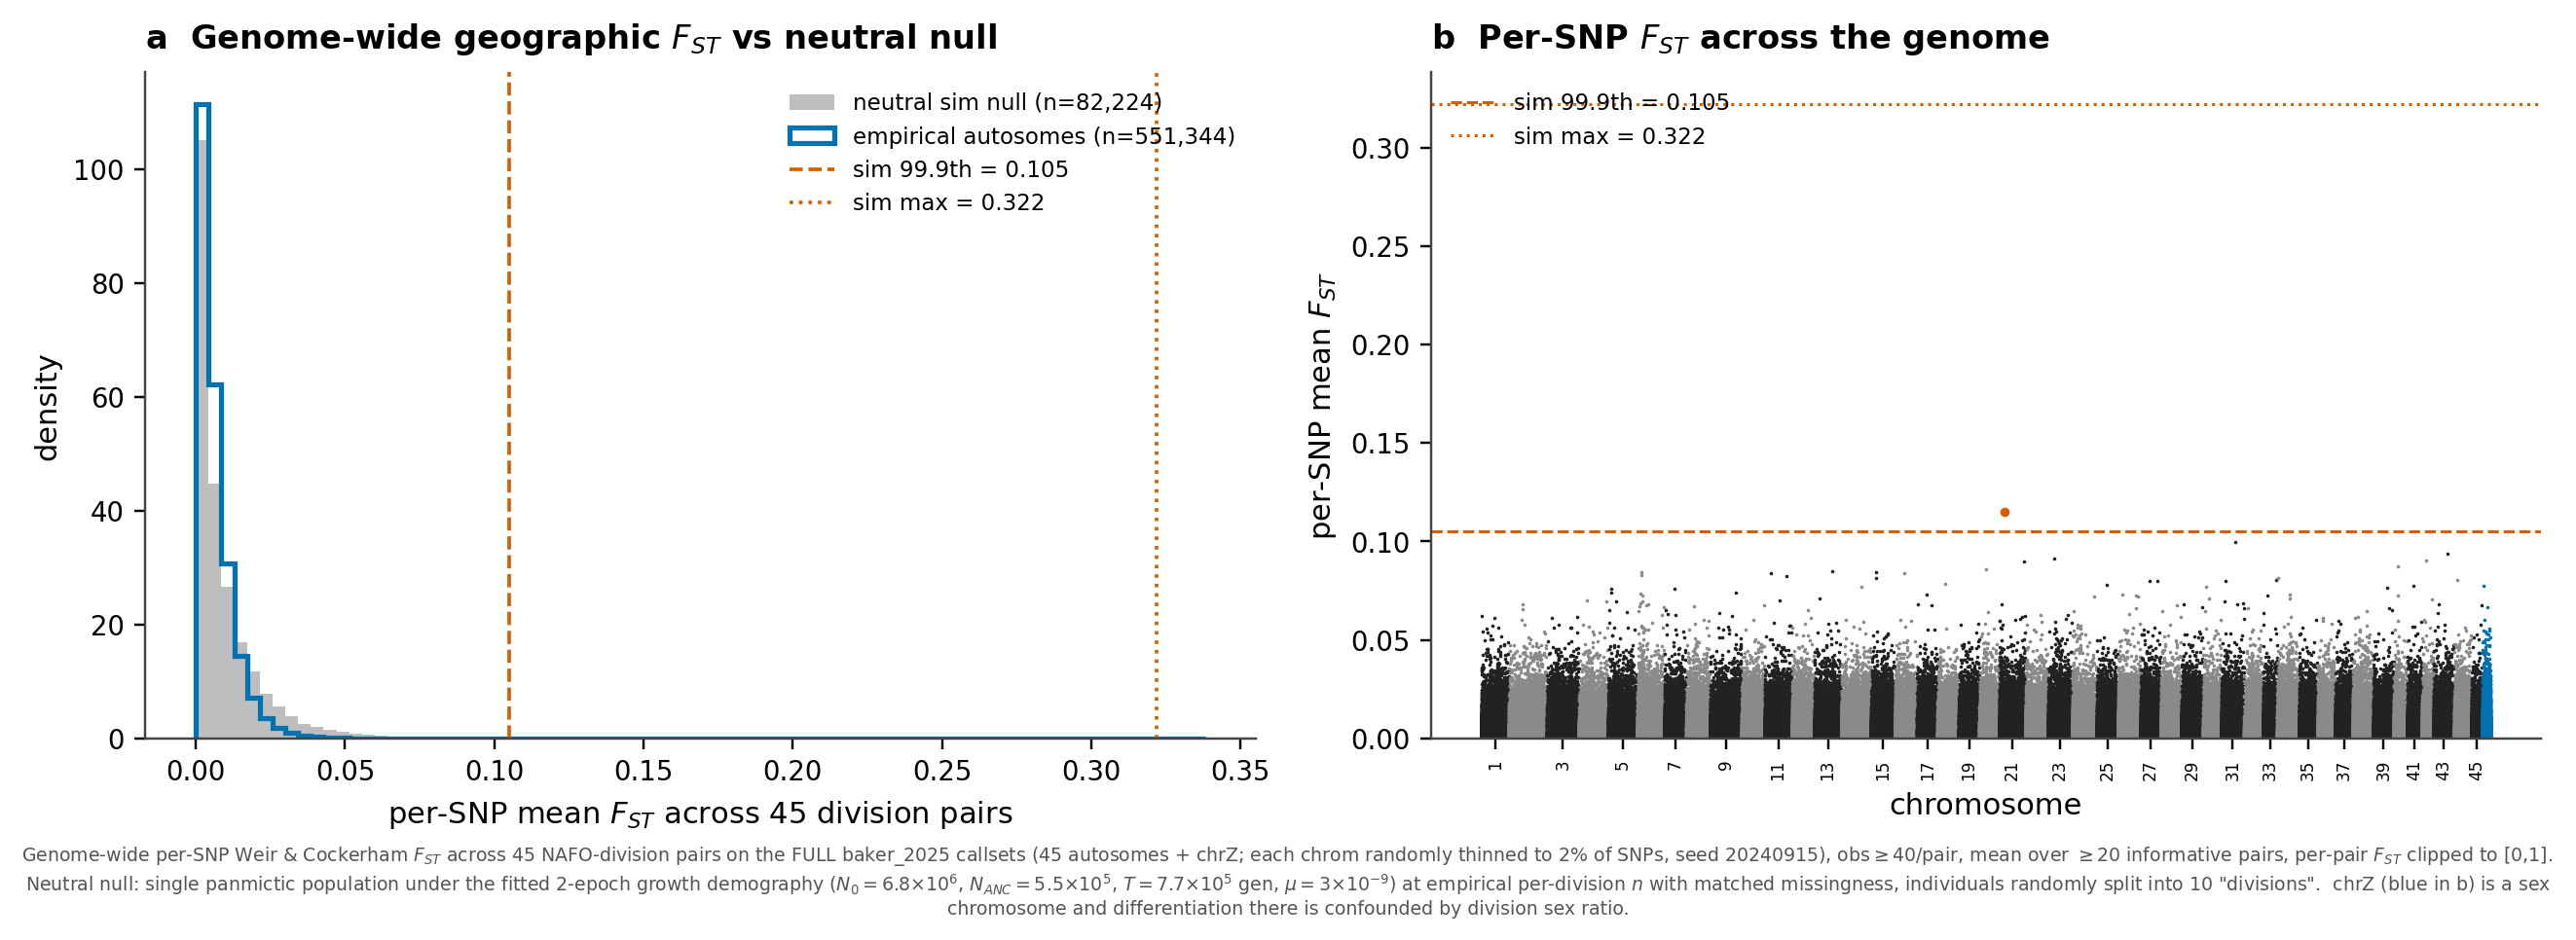
\includegraphics[width=\linewidth]{figS19_fst_genomewide.png}
  \caption{\textbf{Genome-wide per-SNP $\Fst$ finds no differentiation outlier.} The window scan of
    \cref{sfig:fstsnp} extended to the full per-chromosome callsets (551{,}344 autosomal SNPs, 2\%
    thinning, covering 12{,}007 genes). \textbf{(a)}~The empirical per-SNP $\Fst$ distribution across the 45
    division pairs lies entirely within, and is slightly narrower than, the coalescent neutral null.
    \textbf{(b)}~Genome-wide, no SNP exceeds the neutral maximum ($0.322$); a single intergenic SNP on
    chromosome~21 exceeds the lenient 99.9th percentile ($0.105$), against $\approx$556 expected by chance, i.e.\ $\sim$555$\times$ fewer outliers than the false-positive rate. Zero genic outliers, hence no
    functional enrichment. Extreme panmixia is confirmed at genome scale, and no local-adaptation signal is
    present that the diversity-based sweep scans could have missed. (chrZ, blue in (b), is confounded by
    division sex ratios and shown for completeness.)}
  \label{sfig:fstgw}
\end{figure}

\begin{figure}[h]\centering
  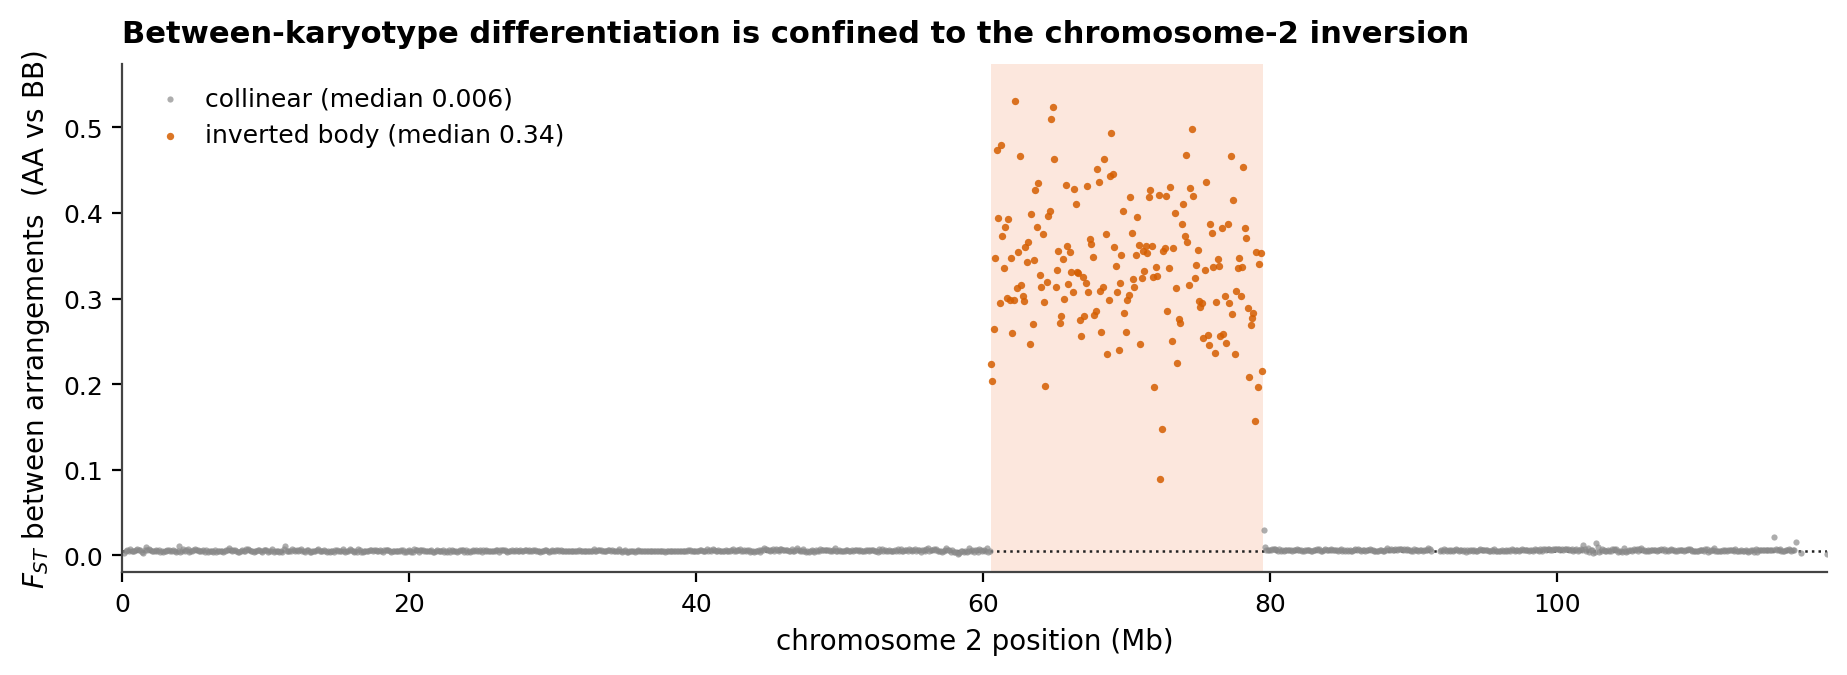
\includegraphics[width=\linewidth]{figS20_chr2_karyotype_fst.png}
  \caption{\textbf{Between-karyotype differentiation is confined to the chromosome-2 inversion.} Per-window
    $\Fst$ between the AA and BB arrangements (arrangement homozygotes, AA $n=254$ and BB $n=95$) across the
    whole of chromosome~2, aggregated in 100~kb windows (ratio-of-averages Hudson estimator). Unlike the
    population-$\Fst$ scan (which asks about geography), this asks how differentiated the two arrangements are
    along the chromosome. The collinear remainder (grey) sits at $\Fst\approx0$ (median 0.006), so outside the inversion the karyotypes are one panmictic population, while the inverted body (60.54--79.50~Mb;
    shaded) is strongly differentiated (median 0.34, max 0.53). The $\Fst\approx0.37$ ``structure'' on
    chromosome~2 is thus between karyotypes and confined to the inversion, not geographic.}
  \label{sfig:karyofst}
\end{figure}

\begin{figure}[h]\centering
  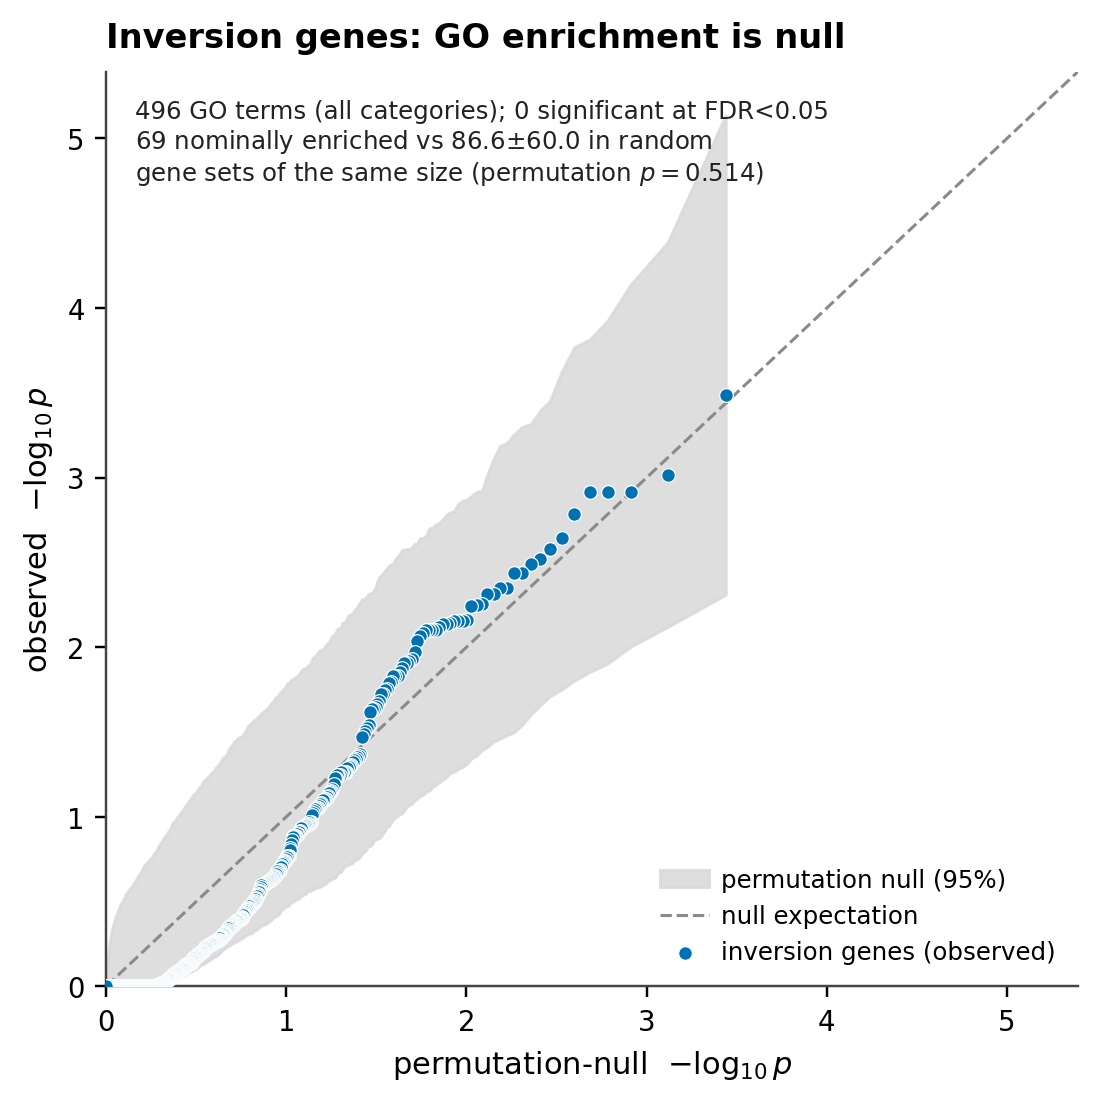
\includegraphics[width=.62\linewidth]{figS21_inversion_go_qq.png}
  \caption{\textbf{The inversion-captured genes show no GO enrichment.} QQ-plot of the per-term GO-enrichment
    $p$-values (Fisher's exact vs.\ genome background, all three ontologies) for the genes in the inversion
    body against a permutation null (500 random gene sets of the same size). A theoretical-uniform
    null is inappropriate for GO, because nested and correlated terms and tiny discrete counts inflate any small gene set, so the permutation band is the correct reference. The observed points fall entirely within it, and the inversion genes yield fewer nominally enriched terms than random sets of the same size
    (69 vs $86.6\pm60$; permutation $p=0.51$) and none survive FDR$<$0.05. The large per-term fold values
    (up to $\sim$40$\times$) are small-count artefacts (most rest on 2 of the 29 GO-annotated genes), not
    enrichment (\cref{stab:invgenes}).}
  \label{sfig:invqq}
\end{figure}

\begin{figure}[h]\centering
  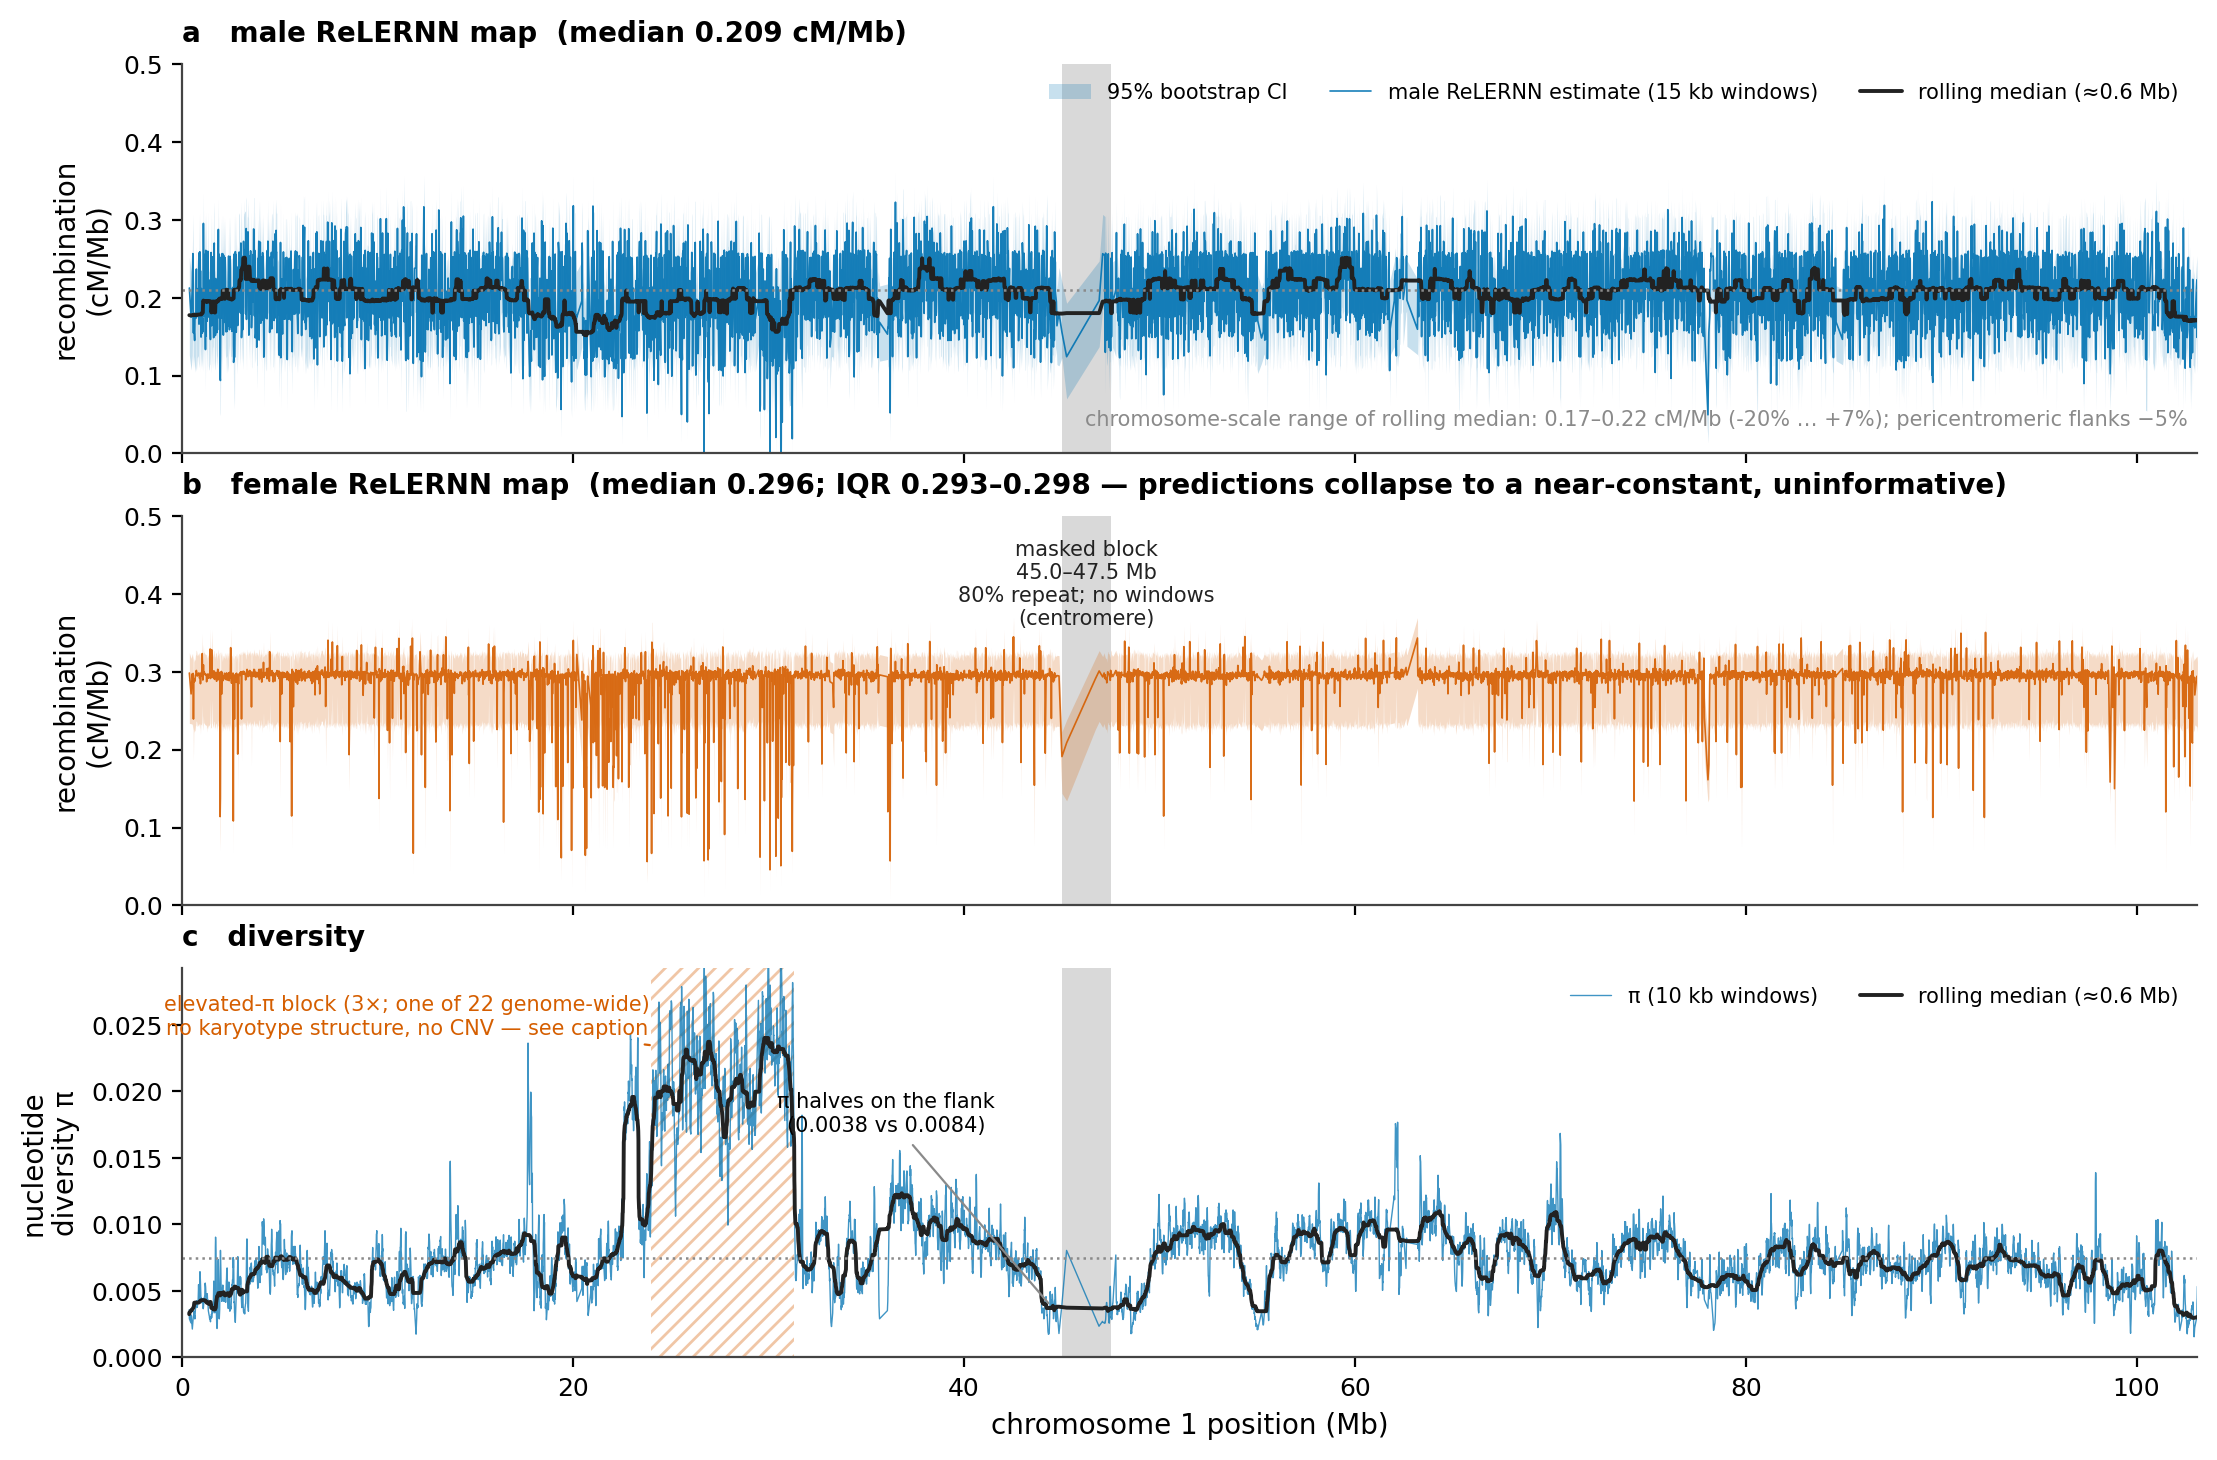
\includegraphics[width=\linewidth]{figS22_chr1_recomb_landscape.png}
  \caption{\textbf{The chromosome-1 recombination map, and what the LD-based map does not resolve.} ReLERNN estimate in 15~kb windows with 95\% bootstrap confidence intervals and a 0.6-Mb rolling median (median 0.209~cM/Mb). The shaded 2.5-Mb block at 45.0--47.5~Mb is 80\% repeat sequence (vs 52\% chromosome-wide), is almost entirely masked, and carries no ReLERNN windows, and it is the centromere. In the accessible pericentromeric flanks the estimate dips only $\sim$5\%, although nucleotide diversity halves there (0.0038 vs 0.0084), and across the whole 103~Mb the rolling median spans just 0.17--0.23~cM/Mb ($-20\%$ to $+7\%$ of the median). The map's chromosome-scale dynamic range is therefore compressed, so centromeric suppression cannot be resolved and the nearly uniform landscape is in part an estimator ceiling.}
  \label{sfig:chr1recomb}
\end{figure}

\begin{figure}[h]\centering
  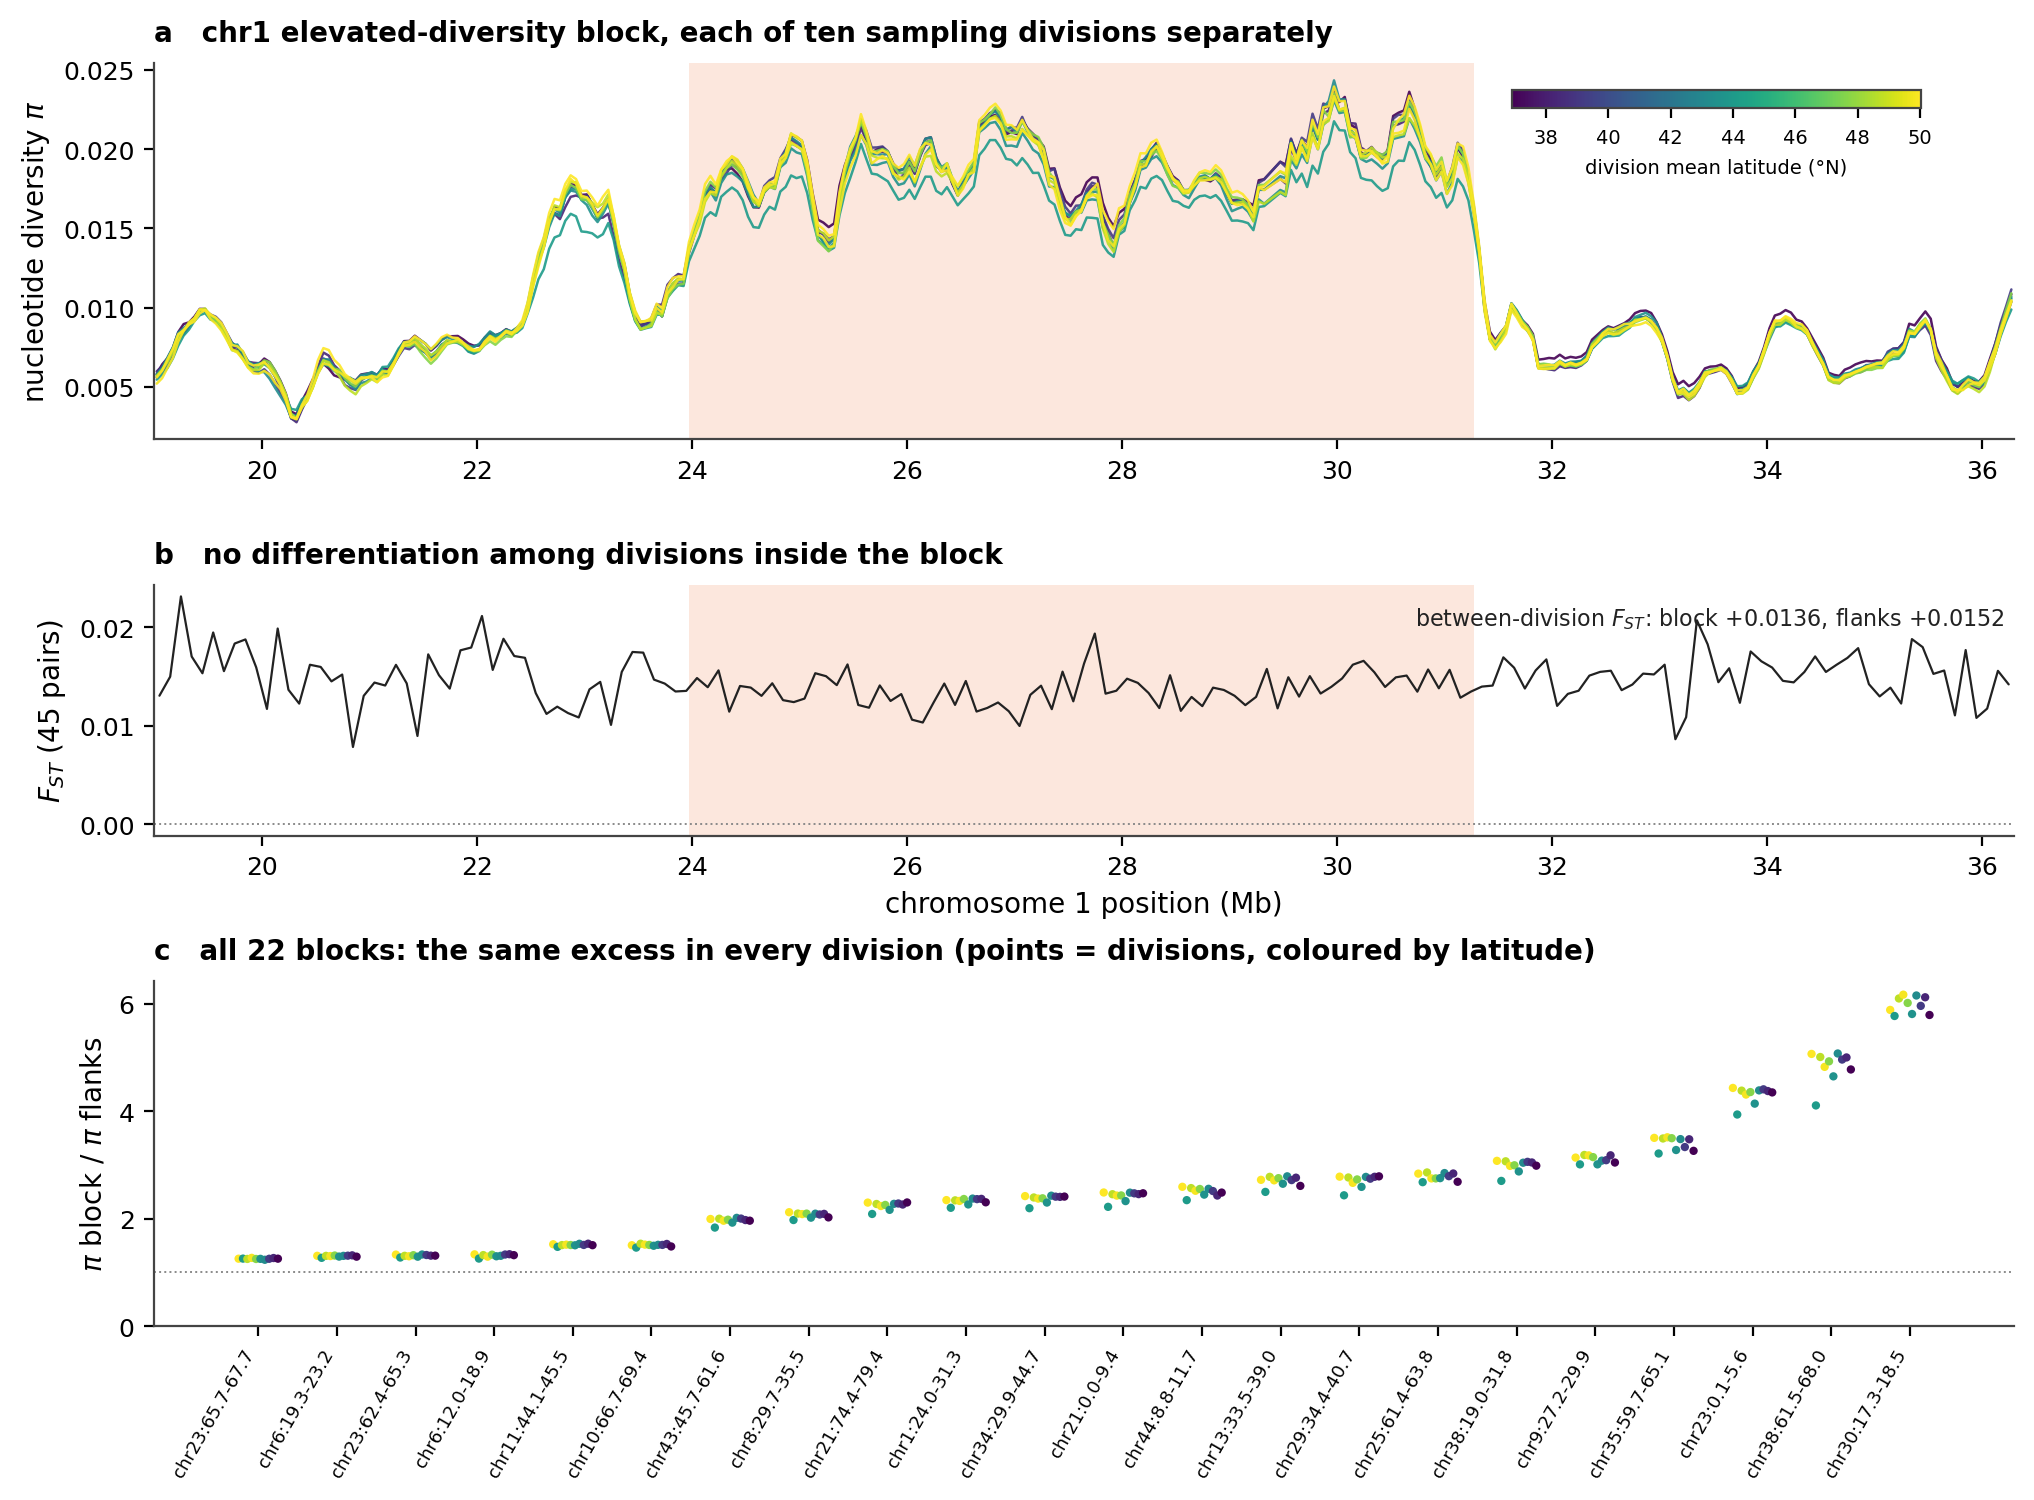
\includegraphics[width=\linewidth]{figS23_pi_blocks_by_division.png}
  \caption{\textbf{The 22 elevated-diversity blocks are shared by every sampling division.} \textbf{(a)}~Nucleotide diversity across chr1:19--36~Mb computed separately in each of the ten divisions with more than one individual (ANGSD, 50-kb windows, lines coloured by division latitude); the 24.0--31.3~Mb block (shaded) carries 2.2--2.4 times the flanking diversity in every division. \textbf{(b)}~Between-division Hudson $\Fst$ over the same span (all 45 division pairs, 100-kb windows) is lower inside the block than in the flanks (0.014 vs 0.015); the same holds for the three strongest blocks (chr30:17.3--18.5, chr23:0.1--5.6 and chr38:61.5--68.0~Mb; 0.006--0.007 inside vs 0.014--0.015 outside). \textbf{(c)}~Block-to-flank diversity ratio per division for all 22 blocks. The excess varies by only 1--6\% among divisions, so no block is driven by a subset of the sample. Read depth separates the blocks into collapsed duplications (depth raised in every individual, up to 2.2 times the flanks in the population sample and 2.7 and 2.4 times in long reads from the assembly individual and a second individual, with five to six times the flanking density of heterozygous sites at skewed allele fractions in single diploid genomes), under-mapped divergent haplotypes (short-read depth 0.6--0.9 times the flanks, with a much smaller deficit in long reads), and gene-poor regions of elevated diversity with normal depth (Supplementary Table~S9). Genotype-likelihood diversity at mapping quality 60 retains most of the excess (for example chr30 6.4 to 5.8 times, chr23 5.2 to 4.0 times), because reads from unassembled copies map uniquely to the single assembled copy. All 22 blocks are masked from the sweep scan and gene-set analyses.}
  \label{sfig:piblocks}
\end{figure}

\begin{figure}[h]\centering
  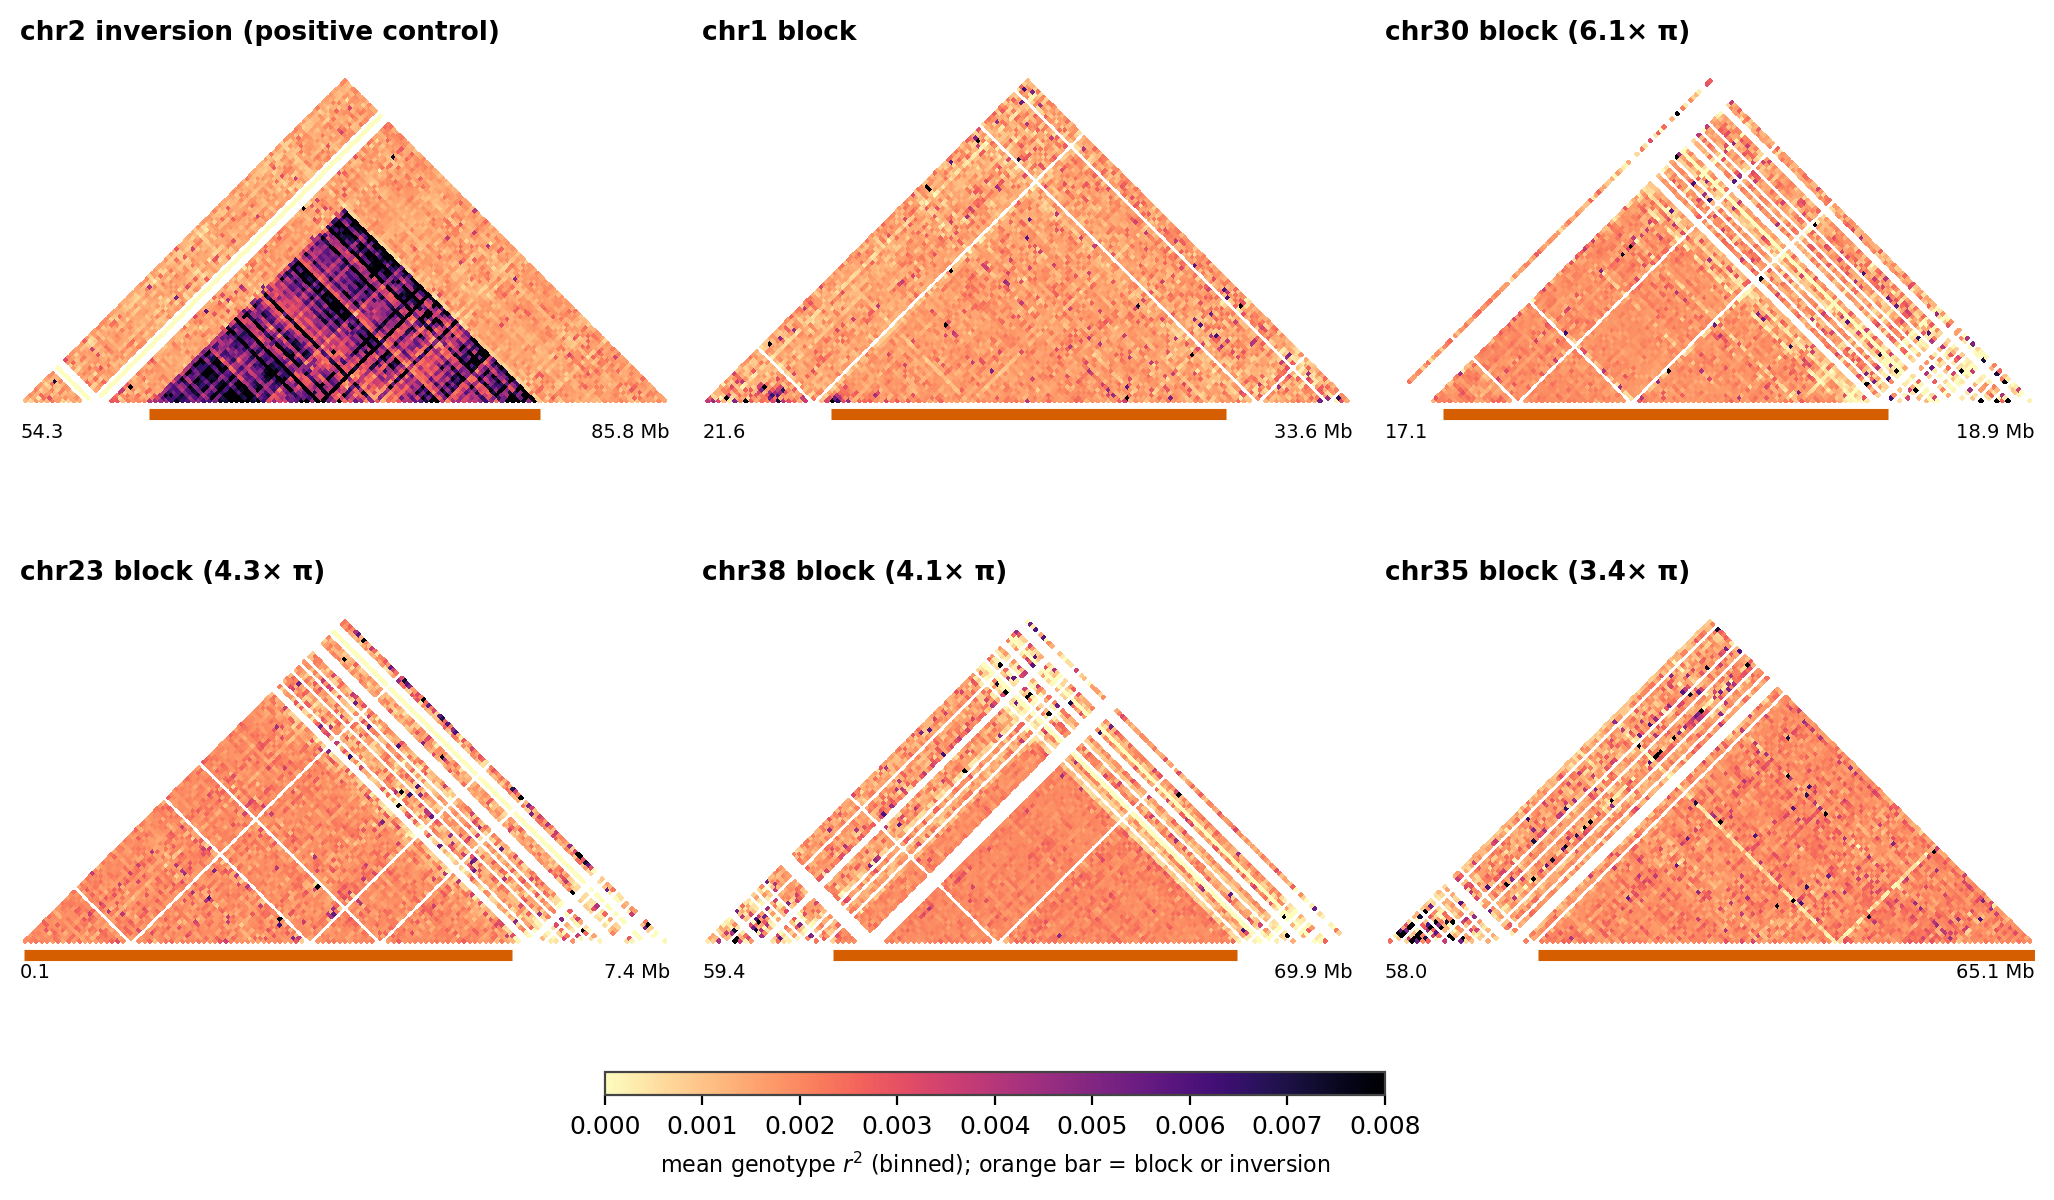
\includegraphics[width=\linewidth]{figS24_block_ld_triangles.png}
  \caption{\textbf{The elevated-diversity blocks carry no inversion-like linkage disequilibrium.} Genotype $r^2$ among common SNPs (minor-allele frequency $\geq$0.1, $\leq$30\% missing; 1{,}500 SNPs per region), averaged in 120 bins, for the chromosome-2 inversion (positive control) and five of the strongest blocks, each shown with a third of its length of flanking sequence; the orange bar marks the inversion or block. The inversion is a solid block of long-range LD over exactly its span (mean $r^2$ at $>$1~Mb 0.0056 inside vs 0.0016 in its flanks). None of the blocks differs from its flanks (0.0017--0.0020 vs 0.0012--0.0021 at $>$1~Mb, across all eight blocks tested), so none behaves as a segregating inversion or other long non-recombining haplotype. White stripes are bins with too few sampled SNPs.}
  \label{sfig:blockld}
\end{figure}



\clearpage
\section*{Supplementary tables}

% ---- S1: software & versions (shared with the Methods) ----
% Software & versions — transcribed from the verified §10 table.
% Included by main.tex via % Software & versions — transcribed from the verified §10 table.
% Included by main.tex via % Software & versions — transcribed from the verified §10 table.
% Included by main.tex via \input{software_table}.
\begin{table}[t]\centering
  \caption{\textbf{Software and versions.} Versions were read off the analysis machine
    (conda metadata, \texttt{pip list}, \texttt{-{}-version}, or recorded \texttt{versions.txt}).
    Citations are pointers to confirm at final formatting.}
  \label{tab:software}
  \small
  \begin{tabular}{lll}
    \toprule
    Tool (version) & Used for & Reference \\
    \midrule
    msinv 0.3.5              & chr2 inversion age/decline (inversion)   & \citep{msinv}; \citep{kelleher2016} \\
    ANGSD 0.940              & SFS, $\theta$, diversity (demography, diversity) & \citep{korneliussen2014angsd} \\
    Stairway Plot 2 (2.1.1)  & demography                 & \citep{liu2020stairway} \\
    GONE2 1.0.4              & recent demography          & \citep{gone2} \\
    moments 1.6.0            & demographic inference (demography)      & \citep{jouganous2017moments} \\
    demes 0.2.3              & demography interchange                         & \citep{gower2022demes} \\
    ReLERNN 0.2              & recombination map         & \citep{adrion2020relernn} \\
    diploSHIC 1.1.0          & sweep scan                 & \citep{kern2018diploshic} \\
    RAiSD (\texttt{0c705a8}) & sweep corroboration (sweep scan)        & \citep{alachiotis2018raisd} \\
    SLiM 5.2                 & forward simulation                            & \citep{haller2019slim} \\
    msprime 1.4.2            & coalescent sim, mutation overlay              & \citep{baumdicker2022} \\
    tskit 1.0.3              & tree-sequence I/O                             & \citep{kelleher2018} \\
    discoal 0.1.7a           & sweep-sim validation                          & \citep{kern2016discoal} \\
    pg\_gpu 0.1.1.dev14      & windowed $\pi$/$\dxy$/$\Fst$, PCA             & \citep{pggpu} \\
    mkado 0.5.0              & McDonald--Kreitman            & \citep{mkado} \\
    DIAMOND 2.1.12           & homology (inversion, sweep scan)    & \citep{buchfink2021diamond} \\
    HMMER 3.4                & Pfam domain screen                            & \citep{eddy2011hmmer} \\
    Pfam-A                   & domain screen                                 & \citep{mistry2021pfam} \\
    AnchorWave 1.2.3         & \coin{}$\leftrightarrow$\illex{} alignment    & \citep{song2022anchorwave} \\
    minimap2 2.29            & alignment                                     & \citep{li2018minimap2} \\
    est-sfs 2.04             & ancestral polarisation                        & \citep{keightley2018estsfs} \\
    degenotate 1.3           & 0-/4-fold degeneracy                          & \citep{degenotate} \\
    bedtools 2.30.0          & interval operations                           & \citep{quinlan2010bedtools} \\
    bcftools/samtools 1.21   & VCF/BAM handling                              & \citep{danecek2021samtools} \\
    EarlGrey 7.0.1           & TE annotation                                 & \citep{baril2024earlgrey} \\
    StringTie 3.0.0          & transcript assembly                           & \citep{kovaka2019stringtie} \\
    SQANTI3                  & Iso-Seq QC                                    & \citep{pardo2024sqanti3} \\
    \bottomrule
  \end{tabular}
\end{table}
.
\begin{table}[t]\centering
  \caption{\textbf{Software and versions.} Versions were read off the analysis machine
    (conda metadata, \texttt{pip list}, \texttt{-{}-version}, or recorded \texttt{versions.txt}).
    Citations are pointers to confirm at final formatting.}
  \label{tab:software}
  \small
  \begin{tabular}{lll}
    \toprule
    Tool (version) & Used for & Reference \\
    \midrule
    msinv 0.3.5              & chr2 inversion age/decline (inversion)   & \citep{msinv}; \citep{kelleher2016} \\
    ANGSD 0.940              & SFS, $\theta$, diversity (demography, diversity) & \citep{korneliussen2014angsd} \\
    Stairway Plot 2 (2.1.1)  & demography                 & \citep{liu2020stairway} \\
    GONE2 1.0.4              & recent demography          & \citep{gone2} \\
    moments 1.6.0            & demographic inference (demography)      & \citep{jouganous2017moments} \\
    demes 0.2.3              & demography interchange                         & \citep{gower2022demes} \\
    ReLERNN 0.2              & recombination map         & \citep{adrion2020relernn} \\
    diploSHIC 1.1.0          & sweep scan                 & \citep{kern2018diploshic} \\
    RAiSD (\texttt{0c705a8}) & sweep corroboration (sweep scan)        & \citep{alachiotis2018raisd} \\
    SLiM 5.2                 & forward simulation                            & \citep{haller2019slim} \\
    msprime 1.4.2            & coalescent sim, mutation overlay              & \citep{baumdicker2022} \\
    tskit 1.0.3              & tree-sequence I/O                             & \citep{kelleher2018} \\
    discoal 0.1.7a           & sweep-sim validation                          & \citep{kern2016discoal} \\
    pg\_gpu 0.1.1.dev14      & windowed $\pi$/$\dxy$/$\Fst$, PCA             & \citep{pggpu} \\
    mkado 0.5.0              & McDonald--Kreitman            & \citep{mkado} \\
    DIAMOND 2.1.12           & homology (inversion, sweep scan)    & \citep{buchfink2021diamond} \\
    HMMER 3.4                & Pfam domain screen                            & \citep{eddy2011hmmer} \\
    Pfam-A                   & domain screen                                 & \citep{mistry2021pfam} \\
    AnchorWave 1.2.3         & \coin{}$\leftrightarrow$\illex{} alignment    & \citep{song2022anchorwave} \\
    minimap2 2.29            & alignment                                     & \citep{li2018minimap2} \\
    est-sfs 2.04             & ancestral polarisation                        & \citep{keightley2018estsfs} \\
    degenotate 1.3           & 0-/4-fold degeneracy                          & \citep{degenotate} \\
    bedtools 2.30.0          & interval operations                           & \citep{quinlan2010bedtools} \\
    bcftools/samtools 1.21   & VCF/BAM handling                              & \citep{danecek2021samtools} \\
    EarlGrey 7.0.1           & TE annotation                                 & \citep{baril2024earlgrey} \\
    StringTie 3.0.0          & transcript assembly                           & \citep{kovaka2019stringtie} \\
    SQANTI3                  & Iso-Seq QC                                    & \citep{pardo2024sqanti3} \\
    \bottomrule
  \end{tabular}
\end{table}
.
\begin{table}[t]\centering
  \caption{\textbf{Software and versions.} Versions were read off the analysis machine
    (conda metadata, \texttt{pip list}, \texttt{-{}-version}, or recorded \texttt{versions.txt}).
    Citations are pointers to confirm at final formatting.}
  \label{tab:software}
  \small
  \begin{tabular}{lll}
    \toprule
    Tool (version) & Used for & Reference \\
    \midrule
    msinv 0.3.5              & chr2 inversion age/decline (inversion)   & \citep{msinv}; \citep{kelleher2016} \\
    ANGSD 0.940              & SFS, $\theta$, diversity (demography, diversity) & \citep{korneliussen2014angsd} \\
    Stairway Plot 2 (2.1.1)  & demography                 & \citep{liu2020stairway} \\
    GONE2 1.0.4              & recent demography          & \citep{gone2} \\
    moments 1.6.0            & demographic inference (demography)      & \citep{jouganous2017moments} \\
    demes 0.2.3              & demography interchange                         & \citep{gower2022demes} \\
    ReLERNN 0.2              & recombination map         & \citep{adrion2020relernn} \\
    diploSHIC 1.1.0          & sweep scan                 & \citep{kern2018diploshic} \\
    RAiSD (\texttt{0c705a8}) & sweep corroboration (sweep scan)        & \citep{alachiotis2018raisd} \\
    SLiM 5.2                 & forward simulation                            & \citep{haller2019slim} \\
    msprime 1.4.2            & coalescent sim, mutation overlay              & \citep{baumdicker2022} \\
    tskit 1.0.3              & tree-sequence I/O                             & \citep{kelleher2018} \\
    discoal 0.1.7a           & sweep-sim validation                          & \citep{kern2016discoal} \\
    pg\_gpu 0.1.1.dev14      & windowed $\pi$/$\dxy$/$\Fst$, PCA             & \citep{pggpu} \\
    mkado 0.5.0              & McDonald--Kreitman            & \citep{mkado} \\
    DIAMOND 2.1.12           & homology (inversion, sweep scan)    & \citep{buchfink2021diamond} \\
    HMMER 3.4                & Pfam domain screen                            & \citep{eddy2011hmmer} \\
    Pfam-A                   & domain screen                                 & \citep{mistry2021pfam} \\
    AnchorWave 1.2.3         & \coin{}$\leftrightarrow$\illex{} alignment    & \citep{song2022anchorwave} \\
    minimap2 2.29            & alignment                                     & \citep{li2018minimap2} \\
    est-sfs 2.04             & ancestral polarisation                        & \citep{keightley2018estsfs} \\
    degenotate 1.3           & 0-/4-fold degeneracy                          & \citep{degenotate} \\
    bedtools 2.30.0          & interval operations                           & \citep{quinlan2010bedtools} \\
    bcftools/samtools 1.21   & VCF/BAM handling                              & \citep{danecek2021samtools} \\
    EarlGrey 7.0.1           & TE annotation                                 & \citep{baril2024earlgrey} \\
    StringTie 3.0.0          & transcript assembly                           & \citep{kovaka2019stringtie} \\
    SQANTI3                  & Iso-Seq QC                                    & \citep{pardo2024sqanti3} \\
    \bottomrule
  \end{tabular}
\end{table}


% ---- S2: karyotype frequency by NAFO division (geography / non-cline) ----
\begin{table}[h]\centering
  \caption{\textbf{Chromosome-2 karyotype counts and inverted-arrangement frequency by NAFO division}
    (ordered by latitude). The inverted (BB) frequency $p_\mathrm{inv}$ shows no latitudinal cline
    (range 0.29--0.46), consistent with geographic $\Fst\approx0$ (\cref{sfig:cline}).}
  \label{stab:geo}
  \begin{tabular}{lrrrrrr}
    \toprule
    Division & AA & AB & BB & $N$ & $p_\mathrm{inv}$ & mean lat.\ ($^\circ$N) \\
    \midrule
    6C & 38 & 40 &  9 &  87 & 0.333 & 36.9 \\
    6B & 34 & 47 & 16 &  97 & 0.407 & 38.3 \\
    6A & 35 & 45 & 15 &  95 & 0.395 & 39.2 \\
    3N &  0 &  0 &  1 &   1 & 1.000 & 43.1 \\
    4X & 42 & 41 & 11 &  94 & 0.335 & 43.2 \\
    4W & 21 & 17 &  9 &  47 & 0.372 & 43.6 \\
    3O &  7 &  7 &  2 &  16 & 0.344 & 44.0 \\
    4T &  7 & 11 &  5 &  23 & 0.457 & 47.7 \\
    4R & 27 & 25 &  4 &  56 & 0.295 & 48.7 \\
    4S &  8 &  4 &  3 &  15 & 0.333 & 49.9 \\
    3K & 35 & 47 & 20 & 102 & 0.426 & 50.0 \\
    \midrule
    Total & 254 & 284 & 95 & 633 & 0.374 & --- \\
    \bottomrule
  \end{tabular}
\end{table}

% ---- S3: coindetii outgroup usage (alignment / polarization / MK) ----
\begin{table}[h]\centering
  \caption{\textbf{Use of the two outgroups.} \coin{} served two roles, ancestral-state polarization of
    the chromosome-2 inversion and the divergence term of the genome-wide McDonald--Kreitman (MK) test, both resting on a single whole-genome \coin$\leftrightarrow$\illex{} AnchorWave alignment.
    \textit{I.\ argentinus} was aligned identically (CDS) and used as a secondary MK outgroup; it yields
    $\sim$9$\times$ fewer fixed coding differences than \coin{} yet has genome-wide $\pi$ indistinguishable
    from \illex{}, marking it as a recently-diverged congener of near-identical diversity.}
  \label{stab:coindetii}
  \small
  \begin{tabular}{llr}
    \toprule
    Step & Quantity & Value \\
    \midrule
    \multicolumn{3}{l}{Alignment (AnchorWave v1.2.3, CDS-anchored)} \\
    \quad & \coin{} substitution sites (genome-wide) & 45{,}722{,}335 \\
    \quad & aligned scaffold identity (inversion body) & 99.2--99.9\% \\
    \midrule
    \multicolumn{3}{l}{Polarization of chr2 karyotypes (est-sfs 2.04 + non-circular subset)} \\
    \quad & diagnostic (AA/BB fixed-difference) sites & 13{,}998 \\
    \quad & \dots\ where \coin$=$\illex{} REF (circular; excluded) & 9{,}680 \ (69.2\%) \\
    \quad & \dots\ where \coin{} carries the ALT (non-circular; used) & 4{,}175 \\
    \quad & polarity from non-circular set & BB derived / AA ancestral \\
    \midrule
    \multicolumn{3}{l}{McDonald--Kreitman test (mkado, \coin{} divergence)} \\
    \quad & genes tested & 20{,}999 \\
    \quad & nonsynonymous / synonymous divergence (Dn / Ds) & 15{,}343 / 13{,}670 \\
    \quad & nonsynonymous / synonymous polymorphism (Pn / Ps) & 468{,}124 / 630{,}949 \\
    \quad & asymptotic $\alpha$ (95\% CI) & 0.642 \ (0.539--3.673) \\
    \midrule
    \multicolumn{3}{l}{I.\ argentinus (secondary MK outgroup; CDS alignment)} \\
    \quad & nonsynonymous / synonymous divergence (Dn / Ds) & 1{,}355 / 1{,}805 \\
    \quad & fixed coding differences (vs \coin{} 29{,}013) & 3{,}160 \ ($\sim$9$\times$ fewer) \\
    \quad & asymptotic $\alpha$ & 0.526 \\
    \quad & genome-wide $\pi$ (ANGSD, 6 autosomes; \illex{} $=0.0093$) & 0.0092 \\
    \bottomrule
  \end{tabular}
\end{table}

% ---- S4: Tier-1 GO enrichment ----
\begin{table}[h]\centering
  \caption{\textbf{Gene-ontology enrichment of the Tier-1 (diploSHIC-only, Markov-corrected) sweep genes.}
    The 623 Tier-1 calls overlap 885 genes (475 GO-annotated); enrichment by Fisher's exact test against the
    annotated-gene background on the scanned chromosomes, Benjamini--Hochberg FDR. 124 biological-process terms
    reach FDR$<$0.05, and representative terms are shown, spanning the two dominant themes (neural development;
    RNA-regulatory/transcriptional control). All are carried by the hard-sweep calls; the soft-sweep gene set
    has no term at FDR$<$0.05. The full machine-readable table is \texttt{hmm\_decode\_masked/tier1\_GO\_enrichment.tsv}.}
  \label{stab:goenrich}
  \begin{tabular}{llrrr}
    \toprule
    GO id & term (biological process) & genes (T1/bg) & fold & FDR \\
    \midrule
    GO:0048699 & generation of neurons & 123/1441 & 1.59 & $2.0\times10^{-4}$ \\
    GO:0022008 & neurogenesis & 125/1508 & 1.54 & $2.6\times10^{-4}$ \\
    GO:0030182 & neuron differentiation & 91/1075 & 1.57 & $1.6\times10^{-3}$ \\
    GO:0030154 & cell differentiation & 186/2548 & 1.36 & $5.4\times10^{-4}$ \\
    GO:0009887 & animal organ morphogenesis & 96/1115 & 1.60 & $8.9\times10^{-4}$ \\
    GO:0050767 & regulation of neurogenesis & 66/693 & 1.77 & $1.3\times10^{-3}$ \\
    GO:0000902 & cell morphogenesis & 72/775 & 1.73 & $1.3\times10^{-3}$ \\
    GO:0007409 & axonogenesis & 45/463 & 1.81 & $1.0\times10^{-2}$ \\
    GO:0048858 & cell projection morphogenesis & 59/609 & 1.80 & $1.6\times10^{-3}$ \\
    GO:0051252 & regulation of RNA metabolic process & 145/1920 & 1.40 & $1.3\times10^{-3}$ \\
    GO:2001141 & regulation of RNA biosynthetic process & 135/1768 & 1.42 & $1.6\times10^{-3}$ \\
    \bottomrule
  \end{tabular}
\end{table}

% ---- S5: GO functional clusters (BGS-robust Tier-1) ----
\begin{table}[h]\centering
  \caption{\textbf{Functional clusters of the background-selection-robust Tier-1 sweep genes.} The 151 enriched biological-process GO terms (FDR$<$0.05) of the BGS-robust set (\cref{sfig:gsea}), grouped
    into functional clusters by term semantics. Neural development and cell morphogenesis/differentiation
    dominate, with RNA-regulatory control and organ development, and a distinct photoreception/sensory
    cluster.}
  \label{stab:goclusters}
  \begin{tabular}{lrll}
    \toprule
    functional cluster & terms & fold range & representative term (min FDR) \\
    \midrule
    Neural development & 21 & 1.6--22.2 & generation of neurons ($3\times10^{-5}$) \\
    Cell morphogenesis \& differentiation & 17 & 1.5--2.2 & cell development ($2\times10^{-5}$) \\
    RNA / transcription regulation & 14 & 1.5--2.1 & reg.\ RNA metabolic process ($9\times10^{-4}$) \\
    Organ / anatomical development & 13 & 1.2--2.5 & system development ($3\times10^{-3}$) \\
    Photoreception / sensory response & 7 & 1.2--5.8 & response to light stimulus ($1\times10^{-4}$) \\
    Other regulation / metabolism & 65 & 1.2--22.2 & reg.\ developmental process \\
    \bottomrule
  \end{tabular}
\end{table}

% ---- S6: Tier-2 cross-method-concordant genes ----
\begin{table}[h]\centering
  \caption{\textbf{Tier-2 (cross-method-concordant) sweep genes.} The 24 genome-wide-scan regions where
    the diploSHIC-HMM sweep signal is independently corroborated by an LD/SFS-footprint method (RAiSD or
    SweepFinder2). Nine regions carry a named protein-coding gene (14 genes, listed); the remaining
    concordant regions are gene deserts or uncharacterised loci. Coordinates in Mb; $\alpha$ and DoS from
    the McDonald--Kreitman test against \textit{I.~coindetii} (`--' where the test is unpowered, i.e.\ too
    few fixed/polymorphic sites). The full candidate set, comprising all 227 diploSHIC-outlier regions, the 24 concordant regions
    and the per-region background-selection test, is provided as machine-readable tables
    (\texttt{outlier\_scan\_45\_masked/\{windows,regions\}.tsv} and the \texttt{concordant} gene/MK/BGS tables).}
  \label{stab:candidates}
  \begin{tabular}{llllrr}
    \toprule
    region (Mb) & sweep & gene & EnTAP best hit & $\alpha$ & DoS \\
    \midrule
    1:20.3 & hard & \textit{Aplnr} & Apelin receptor & 1.00 & +0.17 \\
    1:85.5 & hard & \textit{eif3h} & Eukaryotic translation initiation factor 3 & 0.69 & +0.20 \\
    1:85.5 & hard & \textit{babam1} & BRISC and BRCA1-A complex member 1 & -- & -0.48 \\
    1:85.5 & hard & \textit{ttc39b} & Tetratricopeptide repeat protein 39B & -- & -0.27 \\
    2:84.8 & hard & \textit{NDRG3} & Protein NDRG3 & -- & -0.18 \\
    5:38.0 & hard & \textit{cept1} & Choline/ethanolaminephosphotransferase 1 & -- & -1.00 \\
    5:38.0 & hard & \textit{Arsi} & Arylsulfatase I & -- & -0.25 \\
    6:3.0 & hard & \textit{Rexo1} & RNA exonuclease 1 homolog & -- & -0.53 \\
    13:73.2 & hard & \textit{Rab3} & Ras-related protein Rab-3 & -- & -0.17 \\
    13:73.2 & hard & \textit{hyi} & Putative hydroxypyruvate isomerase & -- & -0.64 \\
    13:73.2 & hard & \textit{Vps28} & Vacuolar protein sorting-associated protein 28 & -- & -- \\
    32:9.3 & soft & \textit{Macrod2} & ADP-ribose glycohydrolase MACROD2 & -- & -0.59 \\
    33:9.0 & hard & \textit{Tinagl1} & Tubulointerstitial nephritis antigen-like & -- & -0.23 \\
    35:39.0 & hard & \textit{zag-1} & Zinc finger E-box-binding homeobox (ZEB) & -- & -0.31 \\
    \bottomrule
  \end{tabular}
\end{table}

\clearpage
\begingroup
\footnotesize
\begin{longtable}{llp{72mm}c}
  \caption{\textbf{Genes captured by the chromosome-2 inversion body} (chr2:60.54--79.50~Mb).
    The 45 functionally annotated genes (of 89 gene models), ordered by position; \emph{fixed} $=$
    number of exonic fixed differences between the AA and BB arrangements ($|\Delta\mathrm{AF}|\geq0.9$;
    `--' none). EnTAP best-hit descriptions. The set spans lipid metabolism (phospholipases, PNPLA,
    malonyl-/acyl-CoA transferases), peroxisomal and mitochondrial function, DNA repair
    (XRCC1, TDG, WRNIP1), transcription/splicing (ERG, PRPF8, WDR82) and signalling (PRKCD), with no
    coherent pathway --- consistent with the absent GO enrichment (\cref{sfig:invqq}). Gene IDs are the
    \texttt{LOC\_} suffix.}\label{stab:invgenes}\\
  \toprule
  region (Mb) & gene & EnTAP best hit & fixed \\
  \midrule
  \endfirsthead
  \toprule region (Mb) & gene & EnTAP best hit & fixed \\ \midrule \endhead
  \bottomrule \endfoot
    2:60.6 & \texttt{00005299} & protein HGH1 homolog isoform X1 & -- \\
    2:60.9 & \texttt{00005300} & Phospholipase A2 domain-containing protein & 2 \\
    2:61.4 & \texttt{00005301} & lon protease homolog 2, peroxisomal isoform X2 & -- \\
    2:61.4 & \texttt{00005302} & 39S ribosomal protein L18, mitochondrial & -- \\
    2:61.4 & \texttt{00005303} & sodium- and chloride-dependent taurine transporter & -- \\
    2:61.6 & \texttt{00005304} & cytochrome P450 4X1-like & 4 \\
    2:61.6 & \texttt{00005305} & uncharacterized protein LOC115219520 & -- \\
    2:64.1 & \texttt{00005315} & PNPLA domain-containing protein & -- \\
    2:64.1 & \texttt{00005316} & PNPLA domain-containing protein & -- \\
    2:65.5 & \texttt{00005319} & CCHC-type domain-containing protein & -- \\
    2:65.7 & \texttt{00005320} & uncharacterized protein LOC127831186 & -- \\
    2:66.1 & \texttt{00005322} & solute carrier family 66 member 2 isoform X2 & -- \\
    2:66.3 & \texttt{00005324} & Ubiquitin-conjugating enzyme E2 T & -- \\
    2:68.0 & \texttt{00005330} & PCDHD1 (protocadherin) & -- \\
    2:68.8 & \texttt{00005334} & retrovirus-related Pol polyprotein (transposon) & -- \\
    2:69.0 & \texttt{00005337} & PNPLA domain-containing protein & -- \\
    2:69.0 & \texttt{00005338} & ELMO domain-containing protein & -- \\
    2:69.1 & \texttt{00005339} & malonyl-CoA-acyl carrier protein transacylase, mito. & 1 \\
    2:69.1 & \texttt{00005340} & acidic repeat-containing protein-like & 4 \\
    2:69.1 & \texttt{00005341} & RPGRIP1L (ciliary) & 2 \\
    2:70.2 & \texttt{00005347} & transcriptional regulator ERG homolog & -- \\
    2:71.2 & \texttt{00005349} & transcriptional regulator ERG homolog & -- \\
    2:71.6 & \texttt{00005350} & uncharacterized protein LOC115215517 & 1 \\
    2:71.9 & \texttt{00005351} & cysteine-rich venom protein & 2 \\
    2:72.0 & \texttt{00005352} & cysteine-rich venom protein & -- \\
    2:74.6 & \texttt{00005356} & DUF7043 domain-containing protein & -- \\
    2:77.7 & \texttt{00005360} & SWIM-type domain-containing protein & -- \\
    2:77.8 & \texttt{00005361} & UPB1 ($\beta$-ureidopropionase) & -- \\
    2:77.8 & \texttt{00005362} & DNA-repair protein XRCC1 (N-terminal domain) & -- \\
    2:77.8 & \texttt{00005363} & TIM21 (mitochondrial import) & -- \\
    2:77.9 & \texttt{00005364} & dynein light chain roadblock-type 2 & -- \\
    2:77.9 & \texttt{00005365} & TDG (thymine-DNA glycosylase) & -- \\
    2:78.0 & \texttt{00005367} & small integral membrane protein 4 & -- \\
    2:78.1 & \texttt{00005368} & uncharacterized protein LOC115226124 & -- \\
    2:78.1 & \texttt{00005369} & ATPase WRNIP1-like & -- \\
    2:78.2 & \texttt{00005371} & unnamed protein product (\textit{Sepia}) & 1 \\
    2:78.2 & \texttt{00005372} & PPM1H (protein phosphatase) & -- \\
    2:78.2 & \texttt{00005373} & WDR82 & -- \\
    2:78.2 & \texttt{00005374} & glycerate kinase-like & -- \\
    2:78.4 & \texttt{00005375} & PRKCD (protein kinase C $\delta$) & -- \\
    2:78.6 & \texttt{00005376} & acyl-coenzyme A amino acid N-acyltransferase 1-like & -- \\
    2:78.7 & \texttt{00005378} & uncharacterized protein LOC115226077 & -- \\
    2:78.7 & \texttt{00005379} & PRPF8 (pre-mRNA splicing factor) & -- \\
    2:78.8 & \texttt{00005380} & synaptic vesicle 2-related protein-like & -- \\
    2:79.3 & \texttt{00005384} & unnamed protein product (\textit{Sepia}) & -- \\
\end{longtable}
\endgroup


\begin{longtable}{llllrr}
\caption{\textbf{Sampling events.} Every collection event (NAFO division, date, depth) with its source, the number of individuals analysed in this study (all 633 whole-genome sequenced individuals) and the number retained by \citet{baker2025} after their genotype-missingness filter (540). Divisions are ordered north to south by mean sampling latitude. 4X was bulk-sampled across the division with no per-tow depth or position recorded.}\label{stab:sampling}\\
\toprule
Division & Date & Source & Depth (m) & $N$ (this study) & $N$ (Baker) \\
\midrule
\endfirsthead
\toprule
Division & Date & Source & Depth (m) & $N$ (this study) & $N$ (Baker) \\
\midrule
\endhead
3K & 16 August 2023 & Recreational jig & 3 & 48 & 48 \\
 & 30 August 2023 & Coastal fishery jig & 5 & 54 & 46 \\
4S & 28 August 2023 & Canadian trawl survey & 228 & 2 & 2 \\
 & 29 August 2023 & Canadian trawl survey & 251 & 1 & 1 \\
 & 30 August 2023 & Canadian trawl survey & 80 & 1 & 1 \\
 & 30 August 2023 & Canadian trawl survey & 124 & 2 & 2 \\
 & 31 August 2023 & Canadian trawl survey & 152 & 2 & 1 \\
 & 31 August 2023 & Canadian trawl survey & 155 & 3 & 3 \\
 & 1 September 2023 & Canadian trawl survey & 273 & 1 & 1 \\
 & 1 September 2023 & Canadian trawl survey & 296 & 1 & 1 \\
 & 3 September 2023 & Canadian trawl survey & 243 & 2 & 2 \\
4R & 7 August 2023 & Canadian trawl survey & 113 & 36 & 24 \\
 & 25 August 2023 & Canadian trawl survey & 173 & 2 & 2 \\
 & 25 August 2023 & Canadian trawl survey & 233 & 5 & 4 \\
 & 25 August 2023 & Canadian trawl survey & 245 & 9 & 7 \\
 & 28 August 2023 & Canadian trawl survey & 221 & 4 & 3 \\
4T & 2 September 2023 & Canadian trawl survey & 243 & 1 & 0 \\
 & 7 September 2023 & Canadian trawl survey & 27 & 1 & 1 \\
 & 8 September 2023 & Canadian trawl survey & 49 & 1 & 0 \\
 & 9 September 2023 & Canadian trawl survey & 112 & 1 & 0 \\
 & 9 September 2023 & Canadian trawl survey & 183 & 1 & 0 \\
 & 9 September 2023 & Canadian trawl survey & 306 & 1 & 0 \\
 & 10 September 2023 & Canadian trawl survey & 81 & 1 & 1 \\
 & 10 September 2023 & Canadian trawl survey & 101 & 1 & 1 \\
 & 10 September 2023 & Canadian trawl survey & 285 & 1 & 0 \\
 & 12 September 2023 & Canadian trawl survey & 285 & 1 & 0 \\
 & 15 September 2023 & Canadian trawl survey & 50 & 1 & 1 \\
 & 22 September 2023 & Canadian trawl survey & 39 & 1 & 1 \\
 & 22 September 2023 & Canadian trawl survey & 142 & 2 & 1 \\
 & 22 September 2023 & Canadian trawl survey & 158 & 1 & 1 \\
 & 23 September 2023 & Canadian trawl survey & 341 & 2 & 2 \\
 & 24 September 2023 & Canadian trawl survey & 118 & 1 & 0 \\
 & 27 September 2023 & Canadian trawl survey & 36 & 1 & 0 \\
 & 28 September 2023 & Canadian trawl survey & 56 & 1 & 1 \\
 & 28 September 2023 & Canadian trawl survey & 62 & 1 & 1 \\
 & 29 September 2023 & Canadian trawl survey & 49 & 2 & 1 \\
3O & 13 October 2023 & Canadian trawl survey & 204 & 14 & 7 \\
 & 14 October 2023 & Canadian trawl survey & 350 & 1 & 1 \\
 & 14 October 2023 & Canadian trawl survey & 613 & 1 & 1 \\
4W & 16 July 2023 & Canadian trawl survey & 84 & 47 & 43 \\
4X & July 2022 & Canadian trawl survey & not recorded & 94 & 76 \\
3N & 20 October 2023 & Canadian trawl survey & 160 & 1 & 1 \\
6A & 22 September 2022 & US trawl survey & 120 & 95 & 84 \\
6B & 18 June 2023 & Commercial trawl & 74 & 49 & 46 \\
 & 16 August 2023 & Commercial trawl & 201 & 48 & 48 \\
6C & 14 September 2022 & US trawl survey & 307 & 87 & 73 \\
\midrule
Total & & & & 633 & 540 \\
\bottomrule
\end{longtable}


\begin{table}[h]\centering\small
\caption{\textbf{Elevated-diversity blocks.} Blocks of $\geq$1~Mb whose rolling nucleotide diversity exceeds twice the chromosome median. $\pi$ fold: block mean over chromosome median. Genes per Mb from the annotation. Division ratio: range across the ten sampling divisions of block-to-flank diversity (5~Mb flanks, ANGSD).}\label{stab:piblocks}
\begin{tabular}{lrrrrrr}
\toprule
Block & Mb & $\pi$ & $\pi$ fold & $D$ block / chrom & Genes/Mb block / chrom & Division ratio \\
\midrule
chr1:24.0--31.3 & 7.3 & 0.021 & 2.8 & $-1.77$ / $-2.21$ & 1.8 / 6.1 & 2.20--2.37 \\
chr6:12.0--18.9 & 6.9 & 0.018 & 2.3 & $-1.58$ / $-2.17$ & 1.7 / 6.8 & 1.26--1.34 \\
chr6:19.3--23.2 & 3.9 & 0.019 & 2.4 & $-1.56$ / $-2.17$ & 1.8 / 6.8 & 1.27--1.32 \\
chr8:29.7--35.5 & 5.8 & 0.018 & 2.3 & $-1.97$ / $-2.22$ & 1.7 / 5.4 & 1.97--2.12 \\
chr9:27.2--29.9 & 2.7 & 0.027 & 3.6 & $-1.12$ / $-2.12$ & 2.2 / 6.5 & 3.01--3.19 \\
chr10:66.7--69.4 & 2.7 & 0.018 & 2.1 & $-2.06$ / $-2.26$ & 0.4 / 5.2 & 1.46--1.53 \\
chr11:44.1--45.5 & 1.4 & 0.015 & 2.1 & $-1.83$ / $-2.15$ & 2.1 / 8.4 & 1.48--1.53 \\
chr13:33.5--39.0 & 5.5 & 0.024 & 2.7 & $-1.79$ / $-2.19$ & 3.1 / 5.5 & 2.50--2.79 \\
chr21:0.0--9.4 & 9.4 & 0.024 & 2.6 & $-1.39$ / $-1.94$ & 1.7 / 6.4 & 2.22--2.49 \\
chr21:74.4--79.4 & 5.0 & 0.023 & 2.5 & $-1.42$ / $-1.94$ & 2.0 / 6.4 & 2.09--2.30 \\
chr23:0.1--5.6 & 5.5 & 0.043 & 4.3 & $-0.96$ / $-2.04$ & 2.2 / 5.8 & 3.94--4.43 \\
chr23:62.4--65.3 & 2.9 & 0.023 & 2.3 & $-1.68$ / $-2.04$ & 2.8 / 5.8 & 1.28--1.33 \\
chr23:65.7--67.7 & 2.0 & 0.023 & 2.3 & $-1.73$ / $-2.04$ & 1.5 / 5.8 & 1.23--1.27 \\
chr25:61.4--63.8 & 2.4 & 0.023 & 2.8 & $-1.57$ / $-2.17$ & 2.9 / 6.2 & 2.68--2.86 \\
chr29:34.4--40.7 & 6.3 & 0.023 & 2.6 & $-1.41$ / $-1.97$ & 2.1 / 7.9 & 2.44--2.79 \\
chr30:17.3--18.5 & 1.2 & 0.057 & 6.1 & $-0.69$ / $-2.17$ & 2.5 / 6.4 & 5.77--6.17 \\
chr34:29.9--44.7 & 14.8 & 0.028 & 2.6 & $-1.45$ / $-1.95$ & 1.8 / 5.2 & 2.20--2.43 \\
chr35:59.7--65.1 & 5.4 & 0.033 & 3.4 & $-1.47$ / $-2.13$ & 1.9 / 6.9 & 3.21--3.52 \\
chr38:19.0--31.8 & 12.8 & 0.032 & 2.8 & $-1.41$ / $-1.97$ & 2.2 / 5.2 & 2.70--3.08 \\
chr38:61.5--68.0 & 6.5 & 0.048 & 4.1 & $-1.08$ / $-1.97$ & 2.6 / 5.2 & 4.11--5.08 \\
chr43:45.7--61.6 & 15.9 & 0.029 & 2.4 & $-1.52$ / $-1.84$ & 2.2 / 6.8 & 1.83--2.02 \\
chr44:8.8--11.7 & 2.9 & 0.028 & 2.7 & $-1.27$ / $-1.85$ & 1.4 / 7.3 & 2.35--2.59 \\
\bottomrule
\end{tabular}
\end{table}


\clearpage
\bibliographystyle{plainnat}
\bibliography{references}

\end{document}
